%% 
%% Copyright 2007, 2008, 2009 Elsevier Ltd
%% 
%% This file is part of the 'Elsarticle Bundle'.
%% ---------------------------------------------
%% 
%% It may be distributed under the conditions of the LaTeX Project Public
%% License, either version 1.2 of this license or (at your option) any
%% later version.  The latest version of this license is in
%%    http://www.latex-project.org/lppl.txt
%% and version 1.2 or later is part of all distributions of LaTeX
%% version 1999/12/01 or later.
%% 
%% The list of all files belonging to the 'Elsarticle Bundle' is
%% given in the file `manifest.txt'.
%% 

%% Template article for Elsevier's document class `elsarticle'
%% with numbered style bibliographic references
%% SP 2008/03/01

\documentclass[preprint,12pt]{elsarticle}

%% Use the option review to obtain double line spacing
%% \documentclass[authoryear,preprint,review,12pt]{elsarticle}

%% Use the options 1p,twocolumn; 3p; 3p,twocolumn; 5p; or 5p,twocolumn
%% for a journal layout:
%% \documentclass[final,1p,times]{elsarticle}
%% \documentclass[final,1p,times,twocolumn]{elsarticle}
%% \documentclass[final,3p,times]{elsarticle}
%% \documentclass[final,3p,times,twocolumn]{elsarticle}
%% \documentclass[final,5p,times]{elsarticle}
%% \documentclass[final,5p,times,twocolumn]{elsarticle}

%% For including figures, graphicx.sty has been loaded in
%% elsarticle.cls. If you prefer to use the old commands
%% please give \usepackage{epsfig}

%% The amssymb package provides various useful mathematical symbols
\usepackage{amssymb}
%% The amsthm package provides extended theorem environments
\usepackage{amsthm}
%% Tthe amsmath package provides the "align" environment for nicer equation formatting
\usepackage{amsmath}
%% The package tabls helps in having nicer tables with higher spaces
\usepackage{tabls}
%% The package multirow allows merging together multiple cells vertifcally
\usepackage{multirow}
%% The package subcaption is for helping when using subfigures and their captions
\usepackage{subcaption}
%% This package is used for having nicer tables
\usepackage{booktabs}

\def\bibsection{\section*{References}}
%% The lineno packages adds line numbers. Start line numbering with
%% \begin{linenumbers}, end it with \end{linenumbers}. Or switch it on
%% for the whole article with \linenumbers.
%% \usepackage{lineno}

\journal{Energy}

\begin{document}

\begin{frontmatter}

%% Title, authors and addresses

%% use the tnoteref command within \title for footnotes;
%% use the tnotetext command for theassociated footnote;
%% use the fnref command within \author or \address for footnotes;
%% use the fntext command for theassociated footnote;
%% use the corref command within \author for corresponding author footnotes;
%% use the cortext command for theassociated footnote;
%% use the ead command for the email address,
%% and the form \ead[url] for the home page:
%% \title{Title\tnoteref{label1}}
%% \tnotetext[label1]{}
%% \author{Name\corref{cor1}\fnref{label2}}
%% \ead{email address}
%% \ead[url]{home page}
%% \fntext[label2]{}
%% \cortext[cor1]{}
%% \address{Address\fnref{label3}}
%% \fntext[label3]{}

\title{Energy and exergy analysis of a cruise ship}

%% use optional labels to link authors explicitly to addresses:
%% \author[label1,label2]{}
%% \address[label1]{}
%% \address[label2]{}

\author[EPFL]{Francesco Baldi}
\author[Linnaeus]{Fredrik Ahlgren}
\author[DTU]{Tuong-Van Nguyen}
\author[CTU]{Cecilia Gabrielii}
\author[CTU]{Karin Andersson}

\address[EPFL]{Industrial Process Energy Systems Engineering (IPESE), \'{E}cole Polytechnique F\'{e}d\'{e}rale de Lausanne, 1950, Sion, Switzerland}
\address[Linnaeus]{Kalmar Maritime Academy, Linnaeus University, Kalmar, Sweden}
\address[DTU]{Department of Mechanical Engineering, Technical University of Denmark, Lyngby, Denmark}
\address[CTU]{Department of Mechanics and Maritime Sciences, Chalmers University of technology, Gothenburg, Sweden}

\begin{abstract}
%% Text of abstract

\end{abstract}

\begin{keyword}
%% keywords here, in the form: keyword \sep keyword

%% PACS codes here, in the form: \PACS code \sep code

%% MSC codes here, in the form: \MSC code \sep code
%% or \MSC[2008] code \sep code (2000 is the default)

low carbon shipping \sep energy analysis \sep exergy analysis \sep energy efficiency

\end{keyword}

\end{frontmatter}

%% \linenumbers

%% main text

%% The Appendices part is started with the command \appendix;
%% appendix sections are then done as normal sections
%% \appendix

%% \section{}
%% \label{}

%% If you have bibdatabase file and want bibtex to generate the
%% bibitems, please use
%%
%%  \bibliographystyle{elsarticle-num} 
%%  \bibliography{<your bibdatabase>}

%% else use the following coding to input the bibitems directly in the
%% TeX file.

\section{Introduction} \label{sec:introduction}

\subsection{Background}

CO$_2$ emissions from shipping in 2012 amounted to a total of 949 million tonnes, contributing to 2.7\% of global anthropogenic CO$_2$ emissions \cite{Smith2014}. Although this contribution appears relatively low, the trend is that shipping will play an even greater role in the future due to the increased transport demand according to all IMO future scenarios \cite{Smith2014}. As an example, global transport demand has increased by 3.4\% in 2014, compared to a global GBP growth of 2.5\% the same year, which shows how shipping tends to rise even faster than global economy \cite{UNCTAD2015}. The OECD countries have reduced the CO$_2$ impact from shipping, but a larger amount has been moved to the non-OECD countries [3]. The fact that shipping needs to even further reduce its CO$_2$ emissions in the near future is essential for being able to achieve the goals of maintaining the climate below a 2-degree level in 2050 [4]. 

In addition to considerations related to GHG emissions, an emission control area (ECA) is enforced in the Baltic Sea  by the International Maritime Organisation since January 2015. This ECA stipulates that the fuel used must not contain more than 0.1\% sulphur, therefore requiring the use of more expensive distillate fuels. More generally making shipping sustainable is a challenge that will demand growing attention by the shipping industry \cite{Andersson2016}

In this context, the cruise industry is growing at an even greater pace. Cruise ship passengers have increased from 17.8 million in 2009 to 24.7 million in 2015 \cite{CruiseOutlook2017}, and this growth is expected to continue in the coming years \cite{CruiseOutlook2017}. Cruise travels, with an estimated average of 160 $kg_{CO_2}$ per passenger and per day, are among the most carbon intensive in the whole tourism industry. The contribution of the cruise industry to global CO$_2$ emissions was estimated to 19.3 Mtons annually in 2010 \cite{Eijgelaar2010}.

The cruise industry have also received much attention for its environmental impact other than in terms of GHG emissions. Cruise ships were shown to have a remarkable negative impact on both air \cite{Poplawski2011} and water \cite{Butt2007} quality, and were also pointed as sources of environmental damage from a wider perspective \cite{Brida2009}. The fact that cruise ships tend to operate extensively in highly populated and environmental sensitive areas makes the situation all the more worth of attention.

Altogether, these conditions present a challenge to the shipping companies who attempt to reduce their fuel consumption, environmental impact, and operative costs. A wide range of fuel saving solutions for shipping are available and partially implemented in the existing fleet, both from the design and operational perspective; several specific studies have been conducted on these technologies, and a more detailed treatise would be out of the scope of this work. In this context, it has been acknowledged that the world fleet is heterogeneous, and measures need to be evaluated on a ship-to-ship basis \cite{Bouman2017}. In this process, a deeper understanding of energy use on board of the specific ship is vital.

\subsection{Previous work}

The idea of improving the understanding of the behavior of the energy system of a ship is not new. Most of the work published around this subject relates to the use  of mathematical models of the ship systems. 

Most authors focused on the propulsion part of the problem, as this is often the most relevant energy demand on board. Shi et al. proposed a modeling approach for predicting ship fuel consumption of a cargo/passenger ferry \cite{Shi2009}; Theotokoats and Tzelepis applied a similar procedure to the case of a Handymax product carrier \cite{Theotokatos2015}, similarly to Tillig et al., who also added the dynamic element to their predictive model \cite{Tillig2016}. 

The work referenced above allowed improving the understanding of how many operational (such as the ship's speed) and environmental (such as wave height and wind speed) parameters influence the ship's energy performance. These studies, however, are not based on actual measurements of the ship's operations. Also, they focus entirely on the ship's power demand for propulsion. This is a very reasonable practice for most ship types, given that propulsion represent the largest part of the total energy demand, but does not allow improving the knowledge of the remaining part of the system.

% Data-driven analysis
Other authors filled the gap by both including electric energy demand, and by basing their work on measurements from actual ship operations. The work presented by Thomas et al. \cite{Thomas2010} and Basurko et al. \cite{Basurko2013} shows the application of energy auditing methods to fishing vessels. This approach represents a step forward towards improving the understanding of how energy is used on board during actual ship operations.  

More generally, several authors have highlighted the importance of a detailed knowledge of the ship's operational profile in order to appropriately assess and optimize possible alternatives for improving ship energy efficiency \cite{Banks2013}. Coraddu et al., started from a statistical analysis of measured ship operations and used the aggregated data, together with a computational model of the vessel, to provide a better prediction of the actual ship's operational efficiency \cite{Coraddu2014}. The importance of considering the operational profile was also showed in the case of the optimization of engine-propeller interaction \cite{Baldi2015c}, in the process of retrofitting existing systems \cite{Baldi2015b,Choi2013}, and in ship design \cite{Ghassemi2017,Solem2015}. 

% Heat availability
Heat demand is rarely a subject of concern on board ships, with some notable exceptions. This is due to a combination of generally low demand and high availability from the waste heat of the engines. In a previous publications by the authors, for instance, it is shown that in the case of a product tanker, although the heat demand was estimated to account for roughly 20\% of the total energy demand of the ship on a yearly basis, it only contributes to 4.1\% of the total fuel consumption (contribution of the auxiliary boilers), while the rest of the demand is fulfilled using waste heat \cite{Baldi2015a}.

%% WHR and heat availability
It should be noted that, however, much research effort has been devoted, especially in recent times, to the improvement of the efficiency of ship energy systems by recovering the waste heat available from the engines. With reference to different types of technologies, case studies, and designs,the several authors showed the existance of a quite significant potential for energy saving when WHR systems are employed, ranging from around 1\% for single-pressure steam cycles applied to two-stroke engines \cite{Theotokatos2012} to more complex systems based on ORCs (up to 10\%, \cite{Hountalas2012}) or including the cooling systems as a source of waste heat (over 10\%, \cite{Dimopoulos2012}).  The case of the installation of an ORC on board of the vessel investigated in this study (see Section \ref{sec:met:case}) was presented in \cite{Mondejar2015}, showing a similar potential.

The potential uses for waste heat on board are not limited to improving the efficiency of the power plant. Waste heat is commonly used for fulfilling on board heat demand for spatial heating and freshwater generation \cite{Molland2011,Baldi2015a,Mccarthy1990};  Balaji et al. proposed the use of waste heat for ballast-water systems \cite{Balaji2012}; Salmi et al. suggested its use for adsorption refrigeration systems \cite{Salmi2017}. A detailed review of potential uses for waste heat from marine engines is presented by Shu et al \cite{Shu2013}. 

% Cruise ships
Some ship types constitute notable examples. On cruise ships the heat demand is significantly higher compared to standard cargo ships. Referring to winter conditions, Marty et al. estimated the instantaneous heat demand of a selected cruise ship to reach roughly 23 MW, compared to an estimated peak of 49 MW for propulsion and electric auxiliaries combined \cite{Marty2012}.  


This shows how the heat from the engines should be considered as a potential resource, rather than a waste, and that there is potential for improvement based on the optimal use of these heat sources. The work presented by the authors in \cite{Baldi2016} represent a step in this direction; however, there is the need for an increased detail in the estimation of the heat demand. 

% Exergy analysis
Exergy analysis provides a more accurate estimation of the potential for energy recovery on board. The application of exergy analysis to the case of ship energy systems is, however, still limited. Dimopoulos et al. showed how the process optimizing the WHR system of a container ship can be more efficient if exergy efficiency, rather than energy efficiency, is used as the target of the optimization \cite{Dimopoulos2012}; Baldi et al. also analyzed the exergy flows on board of a product tanker, showing that this allows having a more accurate understanding of what parts of the system show potential for improvement \cite{Baldi2015a}; similar results were obtained by Marty et al., who focused on the power plant of a cruise ship \cite{Marty2016}. Koroglu et al. made a step futher also including advanced exergy analysis in their study \cite{Koroglu2017}.



\subsection{Aim}

Given the existing limitations of the current available information in scientific literature highlighted in the previous section, the objective of this work is the following:
\begin{itemize}
	\item Analyse the demand of a cruise ship in terms of propulsion power, electric power and heat, based on operational measurements. The lack of existing information with reference to the heat demand is considered a particular element of novelty when compared to existing literature in the subject.
	\item Analyse the current efficiency of the system, and potential ways to improve it, by means of applying exergy analysis.
	\item Provide reference operational conditions for further use in the field of energy systems optimization.
\end{itemize}





\section{Method} \label{sec:method}

In this paper, we present the application of energy and exergy analysis (described in section \ref{sec:met:energyExergy}) to a cruise ship. This is done for one specific case study vessel, that is described in detail in Section \ref{sec:met:case}; in Section \ref{sec:met:gathering} we present the specifics of the available information, in particular the measured data and the technical documentation; the specific assumptions and methods used for processing the available information into  energy and exergy flows are specified in Section \ref{sec:met:processing}. In these regards, the estimation of the heat demand is treated in a separate section (Sec. \ref{sec:met:heat}) as it constitutes a particularly challenging task and it is one of the central aspects of this article. 

\subsection{Energy and exergy analysis} \label{sec:met:energyExergy}

\subsubsection{Energy analysis}

\emph{Energy} can be stored, transformed from one form to another (e.g. heat to power) and transferred between systems, but can neither be created nor destroyed (conservation law)~\textbf{Bejan et al.}. The system under study is the \emph{ship energy system} and is thus taken as control volume. The energy balance can be expressed as:

\begin{align}
	\sum_{\mathrm{in}} \dot{H}_{\mathrm{in}} &= \sum_{\mathrm{out}} \dot{H}_{\mathrm{out}} \\
	\dot{H}_{\mathrm{fuel}} + \dot{H}_{\mathrm{air}} &= \sum_{{\mathrm{waste}}}\dot{H}_{{\mathrm{waste}}}+\dot{W}_{\mathrm{el}}+\dot{Q}_{\mathrm{heating}}
\end{align}

The left-hand side term represents, on a time rate basis, the energy associated with the fuel consumed in the boilers and engines ($\dot{H}_{\mathrm{fuel}}$) and the air used in the combustion processes ($\dot{H}_{\mathrm{air}}$). The right-hand side term denotes the power ($\dot{W}_{\mathrm{el}}$) and heat ($\dot{Q}_{\mathrm{heating}}$) required on-site (e.g. propulsion and fuel heating), and the heat discharged into the environment ($\sum_{{\mathrm{waste}}}\dot{H}_{{\mathrm{waste}}}$) with, for instance, the exhaust gases.

The energy flow associated with a material stream is calculated as the sum of the physical and chemical enthalpies, and kinetic and potential energies are neglected.    The physical energy is taken as the relative enthalpy, as underlined in~\textbf{Kotas et al.}, and the chemical energy is taken as the lower/higher heating value. The environmental conditions taken for the present analysis are the ambient pressure and seawater temperature.

\subsubsection{Exergy analysis}

\emph{Exergy} may be defined as the `maximum theoretical useful work (shaft work or electrical work) as the system is brought into complete thermodynamic equilibrium with the thermodynamic environment while the system interacts with it only'~\citep{Moran1989}. Unlike energy, exergy is not conserved but some is destroyed because of the irreversible phenomena taking place in real processes (e.g. chemical reactions like combustion). The exergy balance for the system under study can be expressed as:

\begin{align}
	\sum_{\mathrm{in}} \dot{E}_{\mathrm{in}} &= \sum_{\mathrm{out}} \dot{E}_{\mathrm{out}} +\dot{E}_{d} \\
	\dot{E}_{\mathrm{fuel}} + \dot{E}_{\mathrm{air}} &= \sum_{{\mathrm{waste}}}\dot{E}_{{\mathrm{waste}}}+\dot{E}_{W}+\dot{E}_{Q,\mathrm{heating}}+\dot{E}_{d} 
\end{align}

The left-hand side term represents, on a time rate basis, the exergy associated with the fuel and air. The right-hand side term denotes the exergy of the waste streams, the exergy transfers with heat and power, and the exergy destroyed in the ship system. Kinetic and potential exergies are neglected, and the exergy of a given material stream is derived as the sum of the physical and chemical exergies. The chemical exergy is calculated based on the reference environment of \textbf{Szargut (1989)}, and its value is approximatively equal to the higher heating value for hydrocarbon fuels. The exergy destruction can be calculated from the Gouy-Stodola theorem~\textbf:{Kotas (1995)}.    

The exergy balance may alternatively be formulated as:
\begin{equation}
\dot{E}_{\mathrm{p}} = \dot{E}_{\mathrm{f}} - \dot{E}_{\mathrm{d}} - \dot{E}_{\mathrm{l}} 
\end{equation}

where $\dot{E}_{\mathrm{p}}$ is called the exergy product, and corresponds to the desired output of the system, in exergy terms (for example, the power produced in an engine). $\dot{E}_{\mathrm{f}}$ denotes the exergy fuel, and represents the resources spent to drive the studied process (for instance, the fuel used in a combustion process). The last term $\dot{E}_{\mathrm{l}}$ corresponds to the losses of a system, such as the heat discharged into the environment with cooling water. 

\subsubsection{System performance}

The following indicators are used to evaluate the system performance:
\begin{itemize}
	\item the exergy efficiency $\varepsilon$, defined as the ratio between the exergy product and fuel of a given component or system
	\begin{equation} \varepsilon = \frac{\dot{E}_{\mathrm{p}}}{\dot{E}_{\mathrm{f}}} \end{equation}
	\item the efficiency defect $\lambda$, presented in the work of Kotas, defined as the fraction of the total exergy input destroyed in the successive irreversible processes
	\begin{equation} \lambda = \frac{\dot{E}_{\mathrm{d}}}{\dot{E}_{\mathrm{in,tot}}} \end{equation}
	\item  the irreversibility share $\delta$, suggested in the work of Tsatsaronis, defined as the ratio between the exergy destroyed in the $i$-th component in relation to the exergy destroyed in the entire system
	\begin{equation} \delta_i = \frac{\dot{E}_{\mathrm{d},i}}{\dot{E}_{\mathrm{d,tot}}} \end{equation}
	
\end{itemize}    








\subsection{Case study vessel} \label{sec:met:case}

The energy and exergy analysis are here applied to a specific  cruise ship operating daily cruises in the Baltic Sea between Stockholm and the island of \.{A}land. The ship is 176.9 m long and has a beam of 28.6 m, and has a design speed of 21 knots. The ship was built in Aker Finnyards, Raumo Finland in 2004.

The ship has a capacity of 1800 passengers and has several restaurants, night clubs and bars, as well as saunas and pools. This means that the energy system regarding the heat and electricity demand is more complex than a regular cargo vessel in the same size. Typical ship operations, although they can vary slightly between different days, are represented in Figure \ref{fig:typicalShipOperations}. It should be noted that the ship stops and drifts in open sea during night hours before mooring at its destination in the morning, if allowed by weather conditions.

\begin{figure}
	\centering
	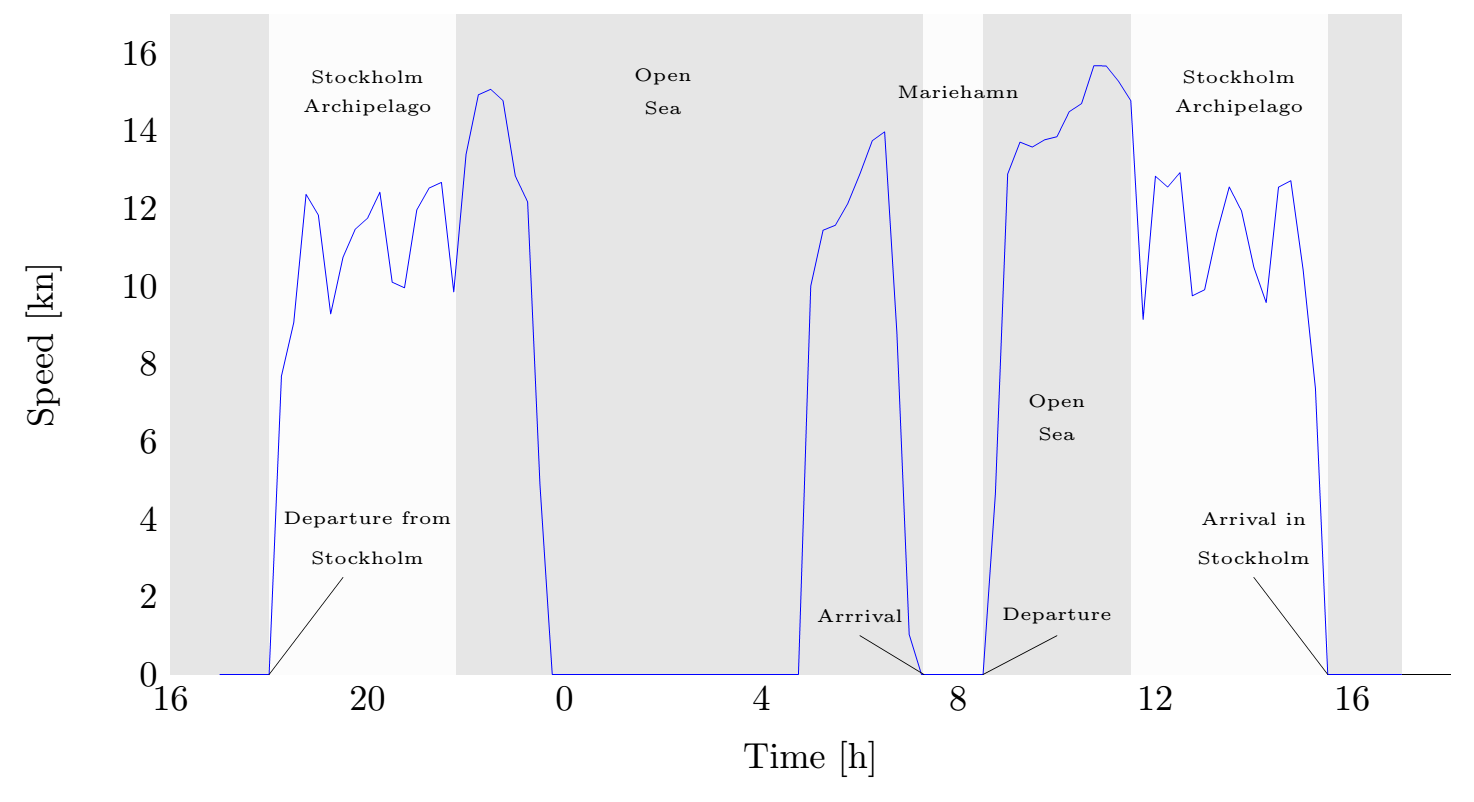
\includegraphics[width=0.95\linewidth]{Figures/ShipOperationalProfile}
	\caption{Reference operational profile (ship speed vs time) for the case study}
	\label{fig:typicalShipOperations}
\end{figure}


The ship systems are summarized in Figure \ref{fig:shipSystems}. The propulsion system is composed of two equal propulsion lines, each made of two engines, a gearbox, and a propeller. The main engines are four W\"{a}rtsil\"{a} 4-stroke Diesel engines (ME) rated 5850 kW each. All engines are equipped with selective catalytic reactors (SCR) for NO$_X$ emissions abatement. Propulsion power is needed whenever the ship is sailing; however, it should be noted that the ship rarely sails at full speed, and most of the time it only needs one or two engines operated simultaneously.

\begin{figure}
	\centering
	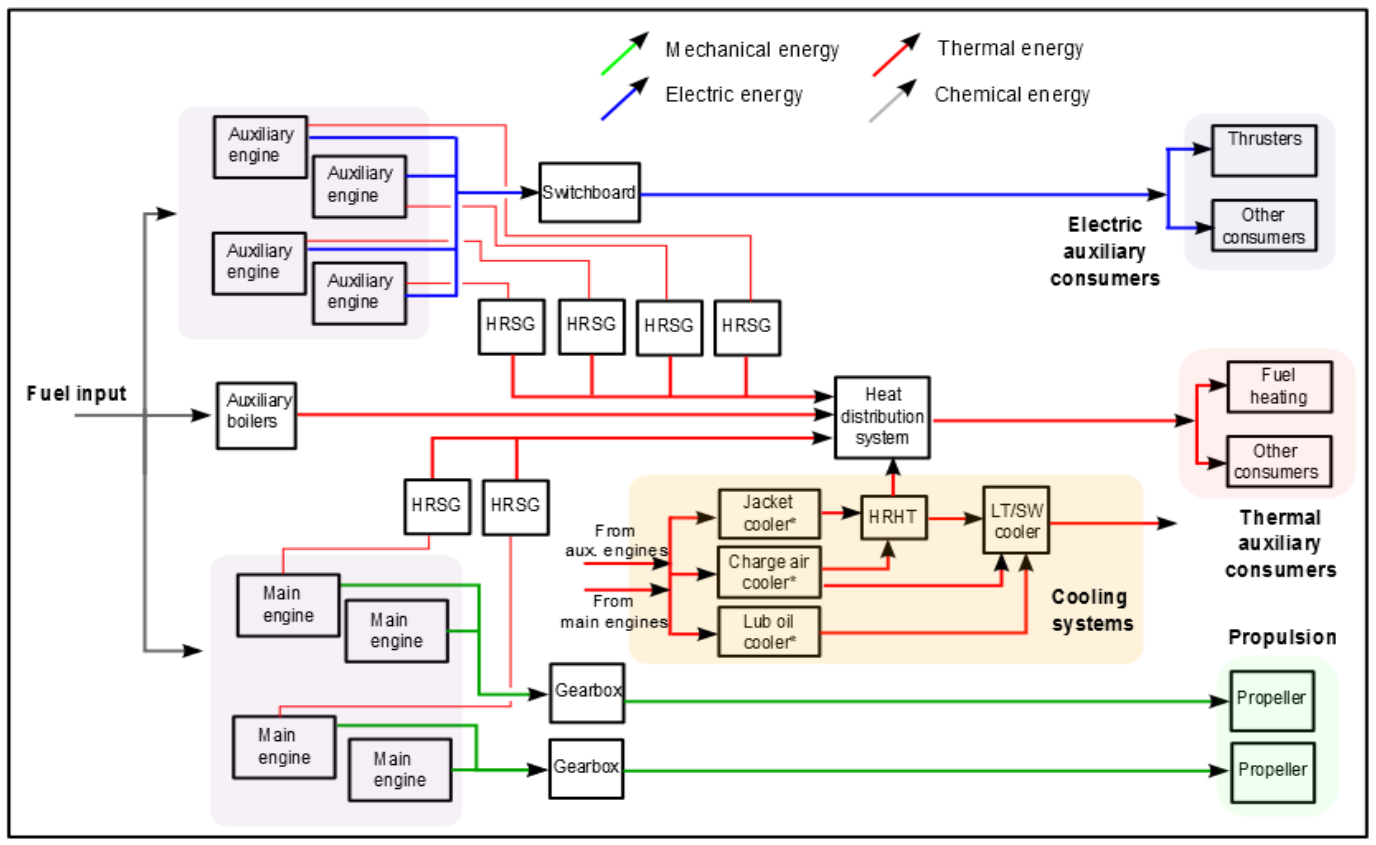
\includegraphics[width=0.95\linewidth]{Figures/ShipLayout}
	\caption{Layout of the case study energy systems}
	\label{fig:shipSystems}
\end{figure}


Auxiliary power is provided by four auxiliary engines (AE) rated 2760 kW each. Auxiliary power is needed on board for a number of alternative functions, from pumps in the engine room to lights, restaurants, ventilation and entertainment for the passengers. 

Auxiliary heat needs are fulfilled by the exhaust gas steam generators (HRSG) located on all four AEs and on two of the four MEs or by oil-fired auxiliary boilers (mainly when in port, or during winter), by the heat recovery on the HT cooling water systems (HRHT), and by the auxiliary, oil fired boilers (AB). The heat is needed for passenger and crew accommodation, as well as for the heating of the highly viscous heavy fuel oil used for engines and boilers. This last part, however, is drastically reduced since the 1st of January 2015, as new regulations entering into force require the use of low-sulphur fuels, which require a much more limited heating.

\subsection{Data gathering and pre-processing} \label{sec:met:gathering}

The operational data was collected on board from the ships' machine logging and surveillance system. The on board database tool exported all logging points to Excel-97 files, and due to the extensive amount of data points the export was divided in to 15 individual Excel-files consisting of a total 665 MB. The exported raw-data from the ship was over a time span of a full year and in most data-points in 15-min average. The Excel-files were processed in the Pandas library which is a high performance data analysis tool in Python \cite{mckinney-proc-scipy-2010}. A new structured naming of headers and a consistent time frequency over all data points were created, and 245 selected data points were saved in a HDF5 table time series database which is the base for the analysis.

All data-points were checked individually by creating a descriptive statistic and a histogram of each data-point. A filter was applied by setting up a pre-defined maximum and minimum value. As we do not know, or had any meaningful way of deriving, each individual sensors placement, sensor type or calibration status all data must be filtered and checked accordingly for outliers or bad data. 


Since measurements of ambient and seawater temperature from onboard logging systems were not available for the whole dataset, we used measurements taken from SMHI database for Landsort lighthouse for the seawater, and the lighthouse Svenska H\"{o}garna for the ambient temperature. The Landsord lighthouse is situated south of the Stockholm archipelago, and the Svenska H\"{o}garna lighthouse is along the ship route, in between the Swedish archipelago and Åland. The assumption was validated based on  June-December period, for which onboard measurements were available. This resulted in a root mean square error of 1.5 K and 1.9 K for the seawater and the ambient temperature respectively, which we considered to be accurate enough for the purpose of this work. The fit the SMHI-data with the rest of the data-set the SMHI data was resampled from 1h for the seawater and 3h for the ambient temperature, to 15min frequency using a linear interpolation.

\subsection{Data processing: Ship energy system modeling} \label{sec:met:processing}

Not all of the variables required to perform a full energy and exergy analysis of the system are available from measurements. In some cases, they are measurable, but not measured (e.g. some temperatures, mass flows, etc.). In other cases, they are simply impossible, or impractical, to measure (e.g. specific enthalpy, specific entropy). For this reason, part of the ship systems needed to be modeled in order to derive the unknown variables. 




\subsubsection{Diesel engines}

The setup of the engines and their connections to the other ship systems are summarized in Figure \ref{fig:DieselEngines} for the main and auxiliary engines, respectively. The most relevant operative values are provided in Tables \ref{tab:ME_values} and \ref{tab:AE_values} and the main energy flows are listed in Tables \ref{tab:ME_flows} and \ref{tab:AE_flows}. It should be noted that, in the case of the main engines, the engine power output was not measured and needed to be estimated. In this work, we calculated the engine power output based on measurements of engine fuel rack position (used as a proxy of the mass of fuel injected per cycle) and of the engine speed:
\begin{eqnarray}
\dot{m}_{fuel} & = & \dot{m}_{fuel,des} \left(a_0 + a_1 \frac{frp}{frp_{des}}\right) \frac{\omega}{\omega_{des}} \\
\eta_{ME} & = & a_0 + a_1 \frac{\dot{m}_{fuel}}{\dot{m}_{fuel,des}} + a_2 \left( \frac{\dot{m}_{fuel}}{\dot{m}_{fuel,des}} \right)^2 \\
\dot{W}_{ME} & = & \dot{m}_{fuel} \eta_{ME} LHV
\end{eqnarray}

The validity of this assumption can be seen by observing Figures \ref{fig:Pme_vs_vship_Neng} and \ref{fig:Pme_vs_TCspeed} where the calculated  power from the main engines is represented against the ship speed and the turbocharger speed, respectively.

\begin{figure}
	\centering
	\includegraphics[width=0.9\linewidth]{Figures/DieselEngines}
	\caption{Schematic representation of the Diesel engines and their connections to the cooling systems}
	\label{fig:DieselEngines}
\end{figure}

In the case of the auxiliary engines, instead, direct measurements of the power generated by each engine were available. 

For both auxiliary and main engines, part of the relevant internal variables are not measured (particularly with relation to the bypass valves) and this required to determine them based on modeling the heat and mass balance of the engine. 
\begin{align}
	\dot{m}_{air,comp} & =  \dot{m}_{air,cyl} + \dot{m}_{air,bp} \label{eq:mb:comp} \\ 
	\dot{m}_{eg,turb} & = \dot{m}_{eg,cyl} + \dot{m}_{air,bp} \label{eq:mb:turb} \\
	\dot{m}_{eg,cyl} & = \dot{m}_{air,cyl} + \dot{m}_{fuel,cyl} \label{eq:mb:cyl} \\
	\dot{m}_{air,comp} \Delta h_{comp} & = \dot{m}_{eg,turb} c_{p,eg} (T_{turb,in} - T_{turb,out}) \eta_{mech} \label{eq:eb:turbocharger} \\
	\dot{m}_{eg,turb} c_{p,eg} (T_{turb,in} - T_0) & = \dot{m}_{air,bp} c_{p,air} (T_{comp,out} - T_0) + \dot{m}_{eg,cyl} c_{p,eg}  (T_{cyl,out} - T_0) \label{eq:eb:bpmerge}
\end{align}
Where equations \ref{eq:mb:comp} to \ref{eq:mb:cyl} represent the mass balances of the bypass split, bypass merge, and cylinder respectively, while equations \ref{eq:eb:turbocharger} and \ref{eq:eb:bpmerge} represent the energy balances of the turbocharger and of the bypass merge, respectively.

The energy balance over the whole engine is presented in Equation \ref{eqn:engineEnergyBalance}.
\begin{equation}
\dot{Q}_{fuel} + \dot{Q}_{air,in} = \dot{W}_{mech} + \dot{Q}_{eg} + \dot{Q}_{cooling}  \label{eqn:engineEnergyBalance} \\
\end{equation}
With: 
\begin{align}
\dot{Q}_{fuel} & =\dot{m}_{fuel} (LHV_{fuel} + c_{p,fuel} (T_{fuel,in} - T_0))\\
\dot{Q}_{air,in} & = \dot{m}_{air} c_{p,air} (T_{air,comp,in} - T_0) \\ 
\dot{Q}_{eg} & = \dot{m}_{eg} c_{p,eg} (T_{eg,TC,out} - T_0) \\
\dot{Q}_{cooling} & = \dot{Q}_{CAC,HT} + \dot{Q}_{CAC,LT} + \dot{Q}_{JWC} + \dot{Q}_{LOC} \label{eq:eb:cooling}
\end{align}

The value of $\dot{Q}_{cooling}$ is determined based on the balance in Equation \ref{eqn:engineEnergyBalance}. The share between the four contributions in Equation \ref{eq:eb:cooling} is calculated based on the data for the heat loss to the HT and LT systems presented in the engines project guides as functions of the engine load. The values are interpolated based on a 2$^nd$ degree polynomial and scaled to respect the energy balance. In absence of more accurate data, it is then assumed that the contributions of $\dot{Q}_{JWC}$ and $\dot{Q}_{LOC}$ are equal for all loads. CHANGE VALUES IN THE TABLE

Values for temperatures, mass flows and energy flows for different engine loads are provided in the Appendix \ref{sec:appendix:engines}, for both main and auxiliary engines.







\subsubsection{Cooling systems}

The ship's cooling systems are designed similarly to most ships and divided in two cooling systems of two separate temperature levels: the high temperature (HT) cooling systems (70-90$^o$C) and the low temperature (LT) cooling systems (40-60$^o$C). The cooling systems provide the necessary cooling to the engines, to the steam systems and to all other components on board. A representation of the ship cooling systems is provided in Figure \ref{fig:generalsystemssimplified}. 

All values not directly measured in the cooling systems were calculated based on mass and energy balances. The mass flow was determined based on measurements of the pressure in the system and on the performance curves of the cooling pumps.

\begin{figure}
	\centering
	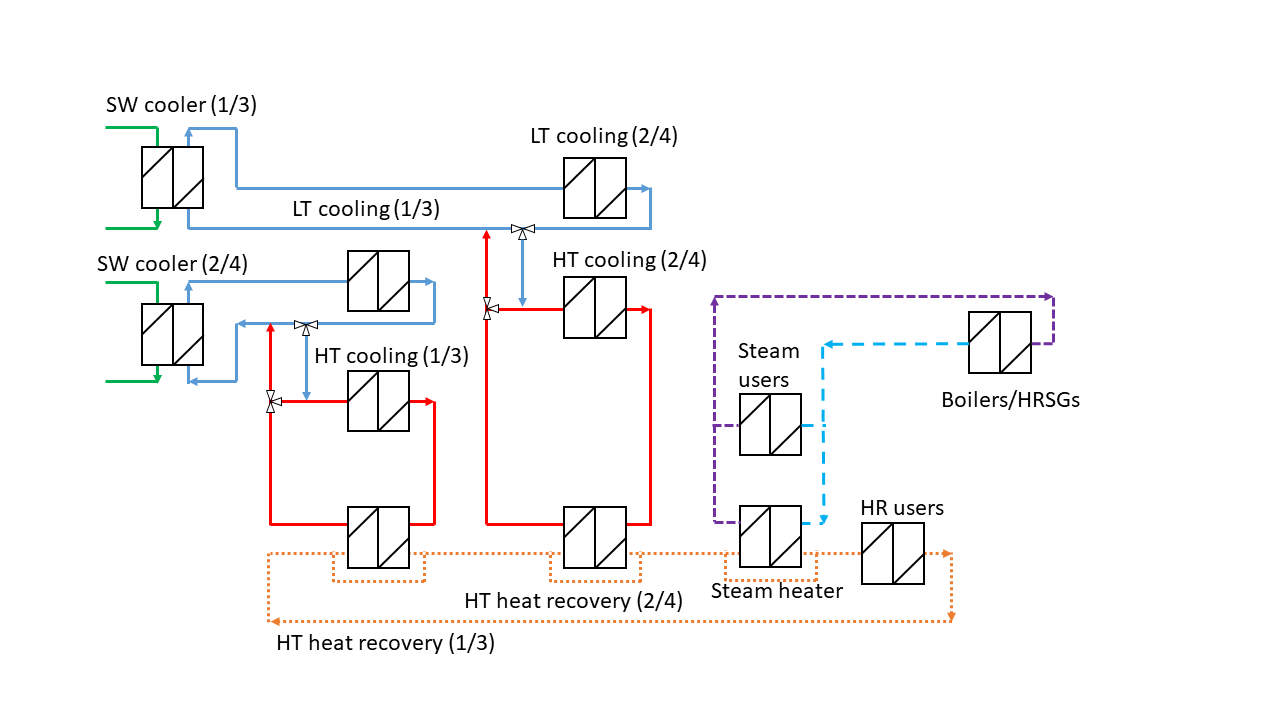
\includegraphics[width=0.9\linewidth]{Figures/GeneralSystemsSimplified}
	\caption{Layout of the ship heating and cooling system}
	\label{fig:generalsystemssimplified}
\end{figure}



\subsection{Electric power demand} \label{sec:met:electric}

The total electric power demand of the system is easily estimated as the sum of the power generated by the four auxiliary engines, that is directly measured on the electrical side of the generators and has a rather high accuracy
\begin{equation}
P_{el,tot} = \sum_{1}^{4} AE_i
\end{equation}

The determination of how different consumers contribute to the total electric power demand is less trivial. The ship is equipped with a number of different systems, including lighting, navigational systems, pumps and compressors, etc. None of the individual contributions is directly measured, hence estimations need to be based on indirect measurements. 

\subsubsection{HVAC systems}

For what concerns the air conditioning unit demand (HVAC), the observation of the total power demand over the year (see Figure \ref{fig:pelvstime}, showing daily averages) leads to the identification of a clear period, corresponding to the summer months, during which there is a significant increase of the demand. 

\begin{figure}
	\centering
	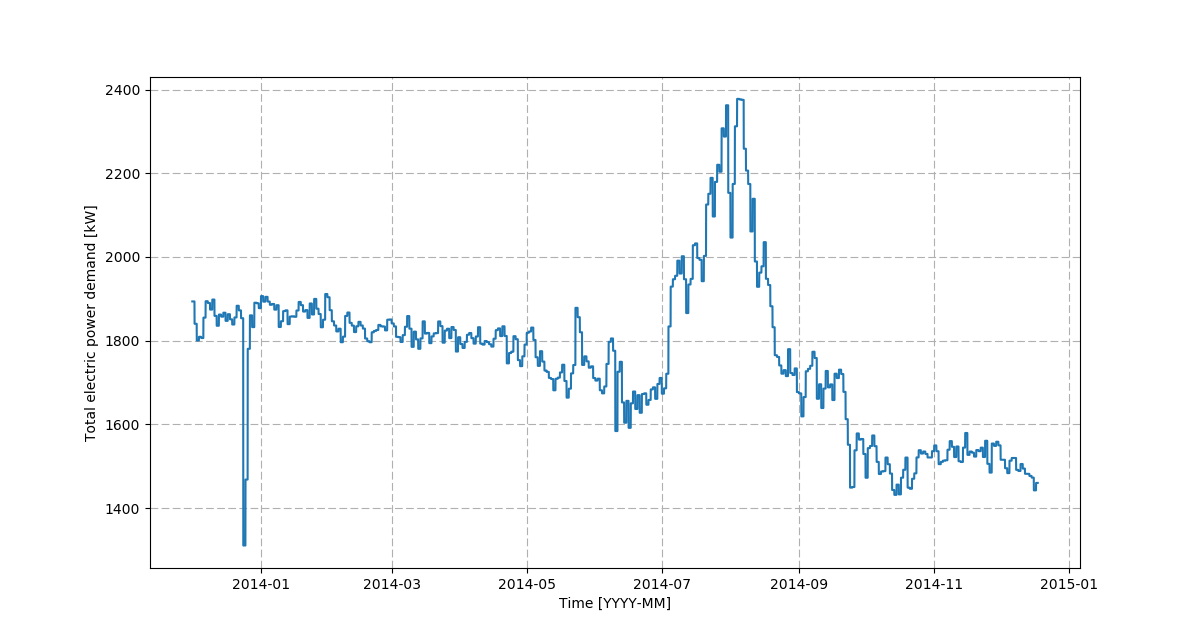
\includegraphics[width=0.9\linewidth]{Figures/Pel_vs_time}
	\caption[Total electric power demand versus time (Daily average)]{Total electric power demand versus time (Daily average)}
	\label{fig:pelvstime}
\end{figure}

Since the total demand seems to be rather constant otherwise, it can be concluded that the demand of the HVAC compressors related to the need for cooling is concentrated during the summer months. Additionally, comparing the evolution of the daily demand (see Figure \ref{fig:pelrelvstime}, representing the instantaneous demand divided by the daily average) between a random summer and winter day, shows that the daily variation is comparable. This shows that assuming a constant consumption for the HVAC during the day does not introduce a substantial error in the estimations.

\begin{figure}
	\centering
	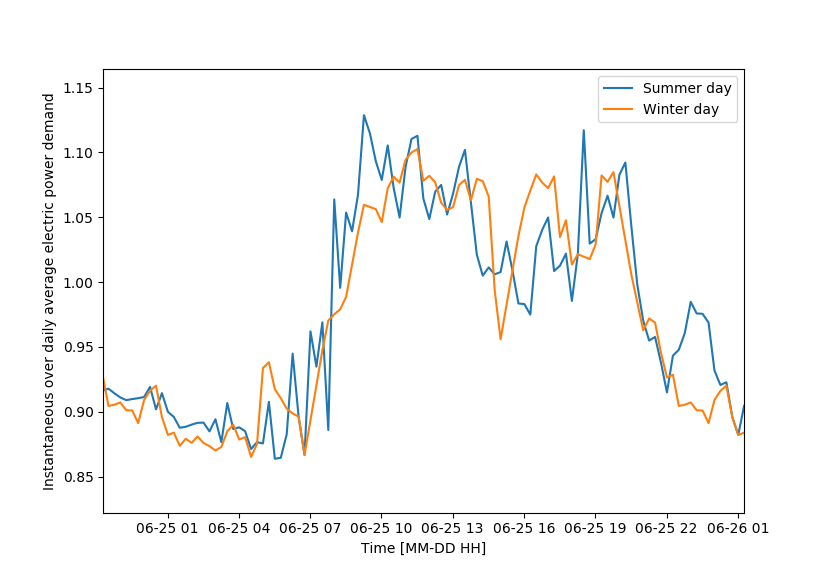
\includegraphics[width=0.9\linewidth]{Figures/PelRel_vs_time}
	\caption{Instantaneous power demand over daily average, winter versus summer day}
	\label{fig:pelrelvstime}
\end{figure}

Hence, the HVAC electric power demand was estimated as follows:
\begin{equation}
P_{el,HVAC} =
\begin{cases}
P_{el,tot}(t) - P_{el,ref}(t) , & \text{if}\ \text{2014-07-03} < t < \text{2014-08-21} \\
0, & \text{otherwise}
\end{cases}
\end{equation}
where $P_{el,ref}(t)$ is calculated as:
\begin{equation}
P_{el,ref}(t) = 0.5 (P_{el,tot}(t_1) + P_{el,tot}(t_2))
\end{equation}


\subsubsection{Thrusters}

When entering port areas, the ship needs to use thrusters to maneuver and berth. In the case of this particular ships, operating on daily schedules and hence maneuvering four times per day, the power demand related to thrusters can be significant. In order to isolate the demand from the thrusters, we created a reference daily energy profile, based on the instantaneous electric power demand divided by the daily average. From this daily profile (made of 96 points), we selected manually selected the points that could be clearly identified as related to the thrusters energy demand, and substituted the actual value with a weighted average of the previous and subsequent points (see Figure \ref{fig:thruster_selection}). 

By comparing the reference profile to the instantaneous one, the points where the former is more than 10\% higher than the latter are identified as "thruster-on" points and treated consequently. 

\begin{figure}
	\centering
	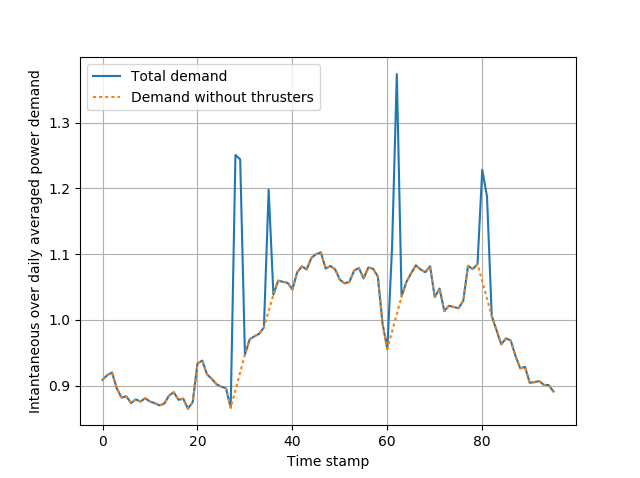
\includegraphics[width=0.9\linewidth]{Figures/Thruster_selection}
	\caption{Example of the procedure of selection of thruster power demand}
	\label{fig:thruster_selection}
\end{figure}



\subsection{Heat demand} \label{sec:met:heat}

As the heat demand is not measured, it is necessary to determine it based on the available indirect measurements. 
	
The heat demand and generation can be summarized according to the following equations:
\begin{eqnarray}
\dot{Q}_{gen} & = & \dot{Q}_{EGB} + \dot{Q}_{HTHR} + \dot{Q}_{AB} \\
\dot{Q}_{dem} & = & \dot{Q}_{HVAC,PH} + \dot{Q}_{HVAC,RH} + \dot{Q}_{HWH} + \dot{Q}_{TH} + \dot{Q}_{G} + \dot{Q}_{OT} + 	\dot{Q}_{HTH} + \dot{Q}_{MSH} \\
\end{eqnarray}

The main view of the ship heating and cooling systems is presented in Figure \ref{fig:ship:general}

\begin{figure}
	\centering
	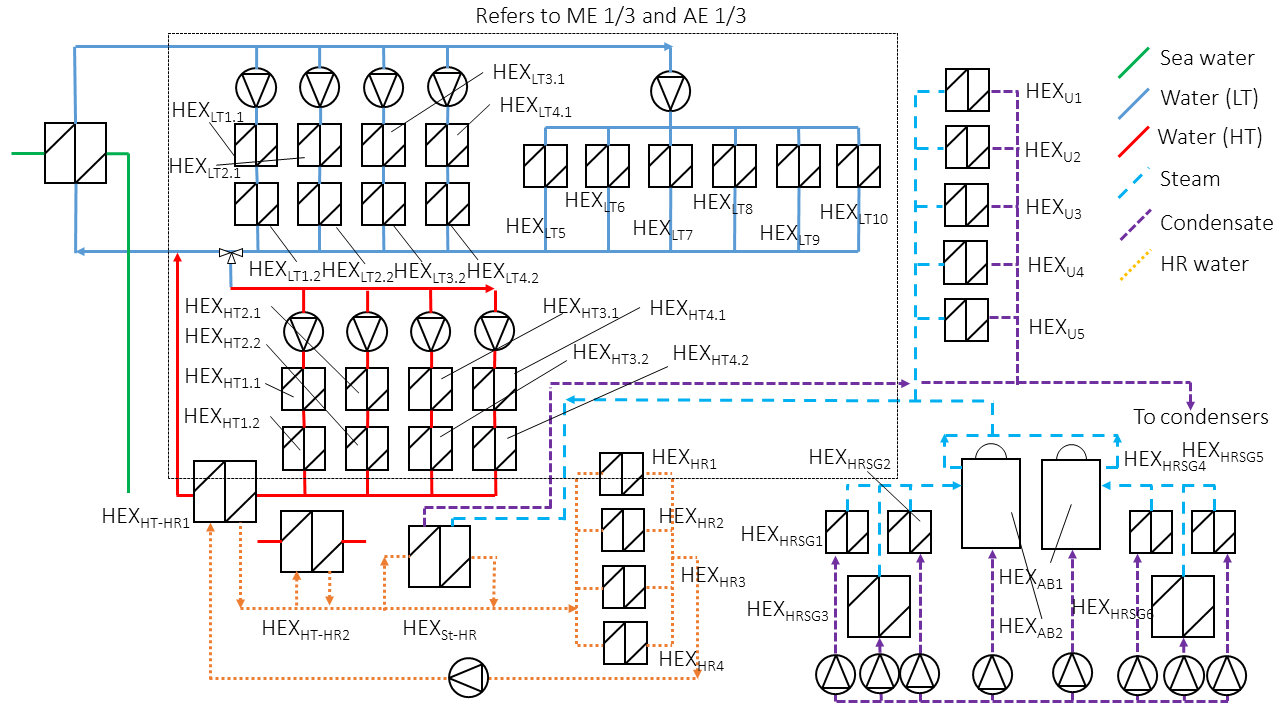
\includegraphics[width=0.999\linewidth]{Figures/Heating_cooling_systems}
	\caption{General view of the ship heating and cooling systems}
	\label{fig:ship:general}
\end{figure}

	
\subsubsection{Heat balance parameter estimation}
	
As not enough information and measurements are available to determine the various components of the heat balance, in this paper we determined them by means of a parameter estimation procedure, using the daily boiler fuel consumption for the calibration of the parameters. The parameter estimation problem is hence written as a minimization problem:
\begin{eqnarray}
min &  \left(\frac{\sum_i(y(\textbf{p})-\bar{y})^2}{\sum_i \bar{y}^2}\right)^{0.5} \\
\end{eqnarray}
	
where the vector $\textbf{p}$ includes the calibration parameters that are part of the heat demand and generation estimation model that is explained in detail in the following sections. A list of the parameters $\textbf{p}$ is shown in Table REF, together with the chosen upper and lower boundaries for the calibration procedure.
\begin{table}
	\centering
	\begin{tabular}{p{3cm}ccp{1.6cm}p{1.6cm}p{1.2cm}}
		\hline 
		Parameter name & Symbol  & Unit & Lower Boundary & Higher Boundary & Optimal value \\ 
		\hline
		Constant HTHR heat demand	 & $\dot{Q}_{k,HTHR}$ & kW & 0 & 1000 &  \\ 
		Constant steam demand		 & $\dot{Q}_{k,steam}$ & kW & 0 & 1000 &  \\
		Weight factor of the HVAC Re-heater & $f_{HVAC,RH}$ & - & 0.5 & 1 &  \\ 
		Weight factor of the HVAC Pre-heater & $f_{HVAC,PH}$ & - & 0 & 1 &  \\ 
		Weight factor of hot water heater & $f_{HWH}$ & - & 0.5 & 1 &  \\ 
		Weight factor of the galley & $f_{G}$ & - & 0.5 & 1 &  \\ 
		Weight factor of the other consumers & $f_{Other}$ & - & 0.5 & 1 &  \\ 
		HTHR inlet temperature & $T_{HTHR,ER1,in}$ & K & 343 & 353 &  \\
		Effectiveness of the HTHR HEX & $\epsilon_{HTHR} $ & - & 0.5 & 0.9 &  \\
		Boiler drum steam storage capacity & $Q_{ab,max}$ & MJ & 100 & 100000 &  \\ 
		Boiler heat rate & $\dot{Q}_{ab,des}$ & kW & 2000 & 8000 &  \\ 
		\hline
	\end{tabular}
	\caption{Parameters optimized in the parameter estimation for the heat balance}
	\label{tab:ParameterEstimation} 
\end{table}
	
	
	
\subsubsection{Heat demand}
	
We calculated the heat demand as the sum of the contributions of the elements listed in the ship's heat balance documentation. As no direct measurement of these quantities was available in the dataset, they had to be estimated based on the following assumptions:
\begin{table}
	\centering
	{\tablinesep=2ex\tabcolsep=10pt
		\begin{tabular}{p{2.8cm}l}
			\hline 
			Heat flow name & Equation \\
			\hline
			HVAC Preheater & $\dot{Q}_{HVAC,PH} = f_{HVAC,RH} \dot{Q}_{HVAC,PH,des} \dfrac{\dot{W}_{HVAC}(t)}{\dot{W}_{HVAC,max}} $ \\
			HVAC Reheater &	$\dot{Q}_{HVAC,RH} = f_{HVAC,PH} \dot{Q}_{HVAC,PH,des} \dfrac{T_{in} - T_{air,out}(t)}{T_{in} - T_{air,out,des}}$ \\
			Hot water heater& $\dot{Q}_{HWH} = f_{HWH} \dot{Q}_{HWH,des} \Phi_{HWH}(\hat{t})$ \\
			Galley & $\dot{Q}_{G} = f_{G} \dot{Q}_{G,des} \Phi_G(\hat{t})$ \\
			Low temperature tank heating & $\dot{Q}_{TH} = f_{TH} \dot{Q}_{TH} \dfrac{T_{T} - T_{air,out}(t)}{T_{T} -T_{air,out,des}}$ \\
			HFO tank heating & $\dot{Q}_{HTH} = f_{HTH} \dot{Q}_{HTH} \dfrac{T_{HT} - T_{air,out}(t)}{T_{HT} - T_{air,out,des}}$ \\
			Machinery space heating & $\dot{Q}_{MSH} = f_{MSH} \dot{Q}_{MSH} \dfrac{T_{MS} - T_{air,out}(t)}{T_{MS} - T_{air,out,des}}$ \\
			HFO heater & $\dot{Q}_{HH} = \dot{m}_{HFO}(t) c_{p,HFO} (T_{HFO,inj} - T_{HT})$ \\
			\hline
	\end{tabular}}
	\caption{Summary of the heat demand contributions and their calculation}
	\label{tab:HeatDemand}
\end{table}
	
where all $f_i$ factors are treated as calibration parameters (see table \ref{tab:ParameterEstimation}). The $\Phi_G(\hat{t})$ and $\Phi_{HWH}(\hat{t})$ functions represent the assumption made on the daily evolution of the heating demand from the galley and the hot water heater respectively. The daily evolutions of the demand are considered to be the same over the whole year of operations and are represented graphically in Figure REF.
	
	
	
\subsubsection{Heat generation}
	
The heat recovered in the EGBs is the only contribution to the heat balance that is known with a reasonable certainty. The heat transferred from the exhaust gas to the steam ($\dot{Q}_{EGB}$) is calculated according to equation \ref{eq:egb}:
\begin{equation}
\dot{Q}_{EGB} = \dot{m}_{eg} c_{p,eg} (T_{eg,EGB,in} - T_{eg,EGB,out})
\end{equation}\label{eq:egb}

where $T_{eg,EGB,out}$ and $T_{eg,EGB,in}$ are measured for all EGBs, $c_{p,eg}$ is calculated as a function of the exhaust gas composition and temperature, and $ \dot{m}_{eg} $ is calculated based on the engine energy and mass balance as described in section REF and in the appendix REF

It is known that the ship heating systems are designed for recovering energy from the high temperature cooling systems of all the ship's engines. However, measurements of this contribution and of other variables that could lead to its straight-forward identification are missing. In this work, we calculated the heat exchanged in the two HTHRs according to equation \label{eqn:HTHR2},

\begin{eqnarray}
\dot{Q}_{HTHR} & = & \dot{Q}_{HTHR,ER1} + \dot{Q}_{HTHR,ER2} \label{eqn:HTHR1} \\
& = & \sum_{i=ER1,ER2}{\epsilon_{HTHR} * \dot{m}_{min,HTHR,i} * c_{p,w} * (T_{HT,out,i} - T_{HRHT,i,in})} \label{eqn:HTHR2}
\end{eqnarray}

where the effectiveness of the heat exchanger $\epsilon_{HTHR}$ is considered to be constant and its value is part of the parameter estimation problem (see table \ref{tab:ParameterEstimation}). The HT water outlet temperature for each engine room is calculated based on the thermal balance of the engines, and the HR water at the HTHR inlet ($T_{HRHT,ER1,in}$) is considered as a calibration parameter. 

The heat generated by the auxiliary boilers is calculated as to close the heat balance of the ship energy systems. The contribution of the boiler heat storage capacity is taken into account by a calibration parameter $Q_{ab,max}$ that determines the maximum heat deficit. This corresponds, in practice, to assuming that the boiler is started up when the steam pressure inside the boiler drops below a certain value, and stopped once the pressure has achieved its maximum operative value. In this calculation, the calibration parameters are the heat storage capacity ($Q_{ab,max}$) and the fixed heat rate ($\dot{Q}_{ab,des}$) of the auxiliary boilers (see table \ref{tab:ParameterEstimation}).





\subsubsection{Parameter estimation and uncertainty quantification}

The results of the parameter estimation are represented graphically and quantitatively in Figure REF and Table REF. 



Given the lack of input values for the estimation of the heat demand, the provided estimate based on the procedure described above should be integrated with an estimation of the uncertainty. 

In this study, we base the estimation of the uncertainty on the production side, as it is the one that has the largest amount of information available. In these regards, the uncertainty can be reduced to the contribution of three elements: $U(\dot{Q}_{EGB})$, $U(\dot{Q}_{HTHR})$, $U(\dot{Q}_{AB})$.

The uncertainty on the heat generated in the EGBs can be further subdivided based on its definition as a composition of the uncertainty of $T_{eg,EGB,in}$, $T_{eg,EGB,out}$, $\dot{m}_{eg}$, and $c_{p,eg}$. In the case of $T_{eg,EGB,in}$ and $T_{eg,EGB,out}$, measured values are used, where the uncertainty is related to the sensors (K-type thermocouples) that can be as high as 4\% [CIT]. The uncertainty on the $\dot{m}_{eg}$ is related to the calculation assumptions as described in Appendix REF, and can be estimated of being up to 10\%. The uncertainty of the $c_{p,eg}$ value, given that both composition and temperature are accounted for, should be within 5\% of the reference value. These assumptions lead to the following estimation of the uncertainty:
\begin{equation}
\frac{\delta \dot{Q}_{gen}}{\dot{Q}_{gen}} = \sqrt{\frac{\delta \dot{m}_{eg}^2}{\dot{m}_{eg}^2} + \frac{\delta c_{p,eg}^2}{c_{p,eg}^2} + \frac{\delta T_{EGB,in}^2 + \delta T_{EGB,out}^2}{(T_{EGB,in} - T_{EGB,out})^2}}
\end{equation}

That once typical values are assigned can be as high as 30\%, where most of the variability is related to the temperature measurements (result obtained for $\pm 20$ K uncertainty. The uncertainty is reduced to 20\% if the measurement uncertainty on the temperature is reduced to  $\pm 20$ K) 

The uncertainty of the heat generated by the ABs can be reduced to the contribution of two elements: the uncertainty on $\dot{m}_{fuel,AB}$ and that on $\eta_{AB}$. The former will be at least as large as the calibration error (35\%) and will be considered equal to 50\% to be conservative and accounting also for errors in the aggregated boiler fuel measurements. In addition, the uncertainty on the efficiency can be considered to be around 10\% based on the discrepancy between the considered sources and on the expected variability of the efficiency with load. Similarly to the previous case, the combination of these efficiencies lead to a total uncertainty of 51\%, where the main contribution comes from the uncertainty of the model output compared to the actual fuel consumption.

The estimation of the uncertainty of $\dot{Q}_{HTHR}$ can be based on \ref{eqn:HTHR2} having assigned an acceptable variation of 20\% to the effectiveness of the heat exchanger, 20\% on the estimation of the reference mass flow, $\pm 5$ K uncertainty on water temperature measurements and considering negligible the uncertainty on $c_{p,w}$, leading to a 145\% uncertainty on this measurement. 


\subsection{Operational mode}

The ship operates in different conditions, and it can be useful to provide a separate analysis depending on the operational mode. The four operational modes identified for the selected case study, together with the conditions applied to the dataset to uniquely identify each time step to a separate operational mode, are given as follows:
\begin{description}
	\item[High speed sailing] Ship speed above 15 kn
	\item[Low speed sailing] Ship speed between 4 and 15 kn
	\item[Maneuvering] Ship speed between 2 and 4 knots OR Thrusters power larger than 0
	\item[Port stays / ship drifting] All other points
\end{description}



\subsection{Determination of typical operational conditions}












\section{Results (and discussion)}

\subsection{Exploratory analysis} \label{sec:res:exploratory}

In this section, we observe and analyze direct measurements from ship systems, with no pre-processing, that are expected to have an influence on the energy analysis.

Figures \ref{fig:TseaTairTIME} and \ref{fig:TseaTairDIST} represent the time evolution and the distribution over the year of the ambient air and sea water temperature. The relatively low temperatures that are experienced by the case study ship during its operations rise expectations for a high space heating demand and to a relatively low for summer HVAC electric power demand. On the other hand, the fact that, in summer, air temperatures reach up to 26 degrees Celsius justify the existence of an HVAC unit that can also operate in cooling mode. 

\begin{figure}[htbp]
	\centering
	\begin{subfigure}[b]{0.45\textwidth}
		\centering
		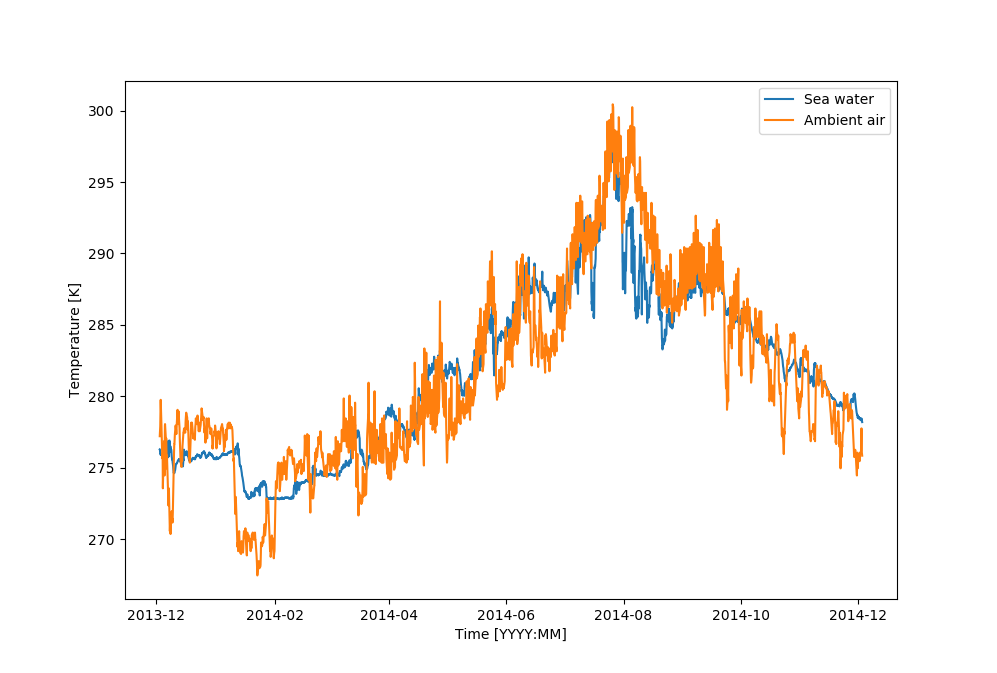
\includegraphics[width=0.999\linewidth]{Figures/Tsea_vs_time}
		\caption{Time series}
		\label{fig:TseaTairTIME}
	\end{subfigure}
	\begin{subfigure}[b]{0.45\textwidth}
		\centering
		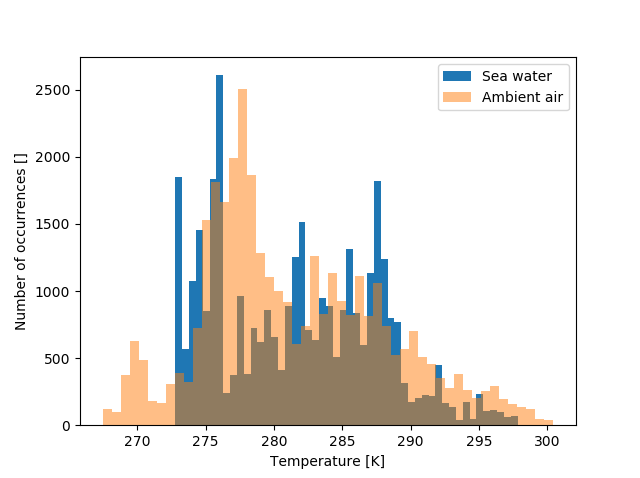
\includegraphics[width=0.9\linewidth]{Figures/Tsea_hist}
		\caption{Distribution}
		\label{fig:TseaTairDIST}
	\end{subfigure}
	\caption{Statistical representation of measured air and sea water temperatures based on yearly data. Landsort, 2014}
	\label{fig:TseaTair}
\end{figure}


Figure \ref{fig:vship_hist} represents the distribution of the ship speed. The ship operates almost for the entire year according to a fix schedule, while there are a couple of periods (particularly during the summer months) when the ship operates at higher speed. In Figure \ref{fig:opMode_pie} it can be also observed that the ship spends a relatively high amount of time in port. These remarks suggest that, in spite of the high installed power of the main engines, the energy demand for propulsion is expected to be relatively low.

Figures \ref{fig:loadME_hist} and \ref{fig:loadME_hist} show the frequency of the load at which each of the engines (main and auxiliary engines, respectively) is operated. In the case of the main engines, it can be observed that they are operated mostly at loads between 30\% and 60\%, despite the optimal load for the engines being located around 85\%. This is a consequence of both the low speed at which the ship is generally operated, and of the fact that the two shaft lines are operated independently, and hence do not allow the use of only one of the four engines at high load. 

In the case of the auxiliary engines, a larger difference between how the engines are operated can be observed. AE-3 is generally more often operated, as it is the engine that is run in port with clean fuels. On the other hand, it seems that AE-4 is operated rarely, which might be due to maintenance issues.

\begin{figure}[htbp]
	\centering
	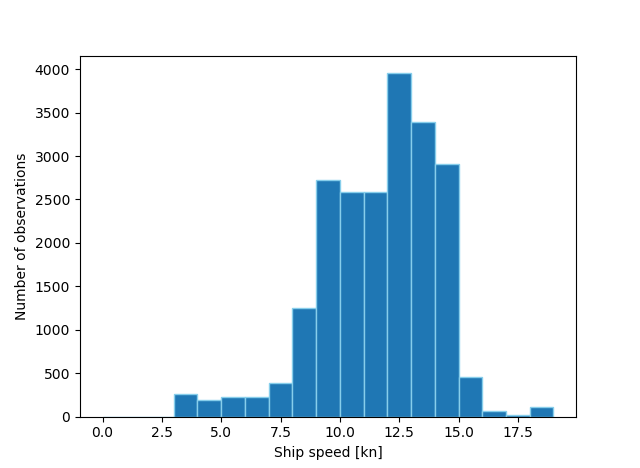
\includegraphics[width=0.8\linewidth]{Figures/vship_hist}
	\caption{Yearly distribution of ship speed}
	\label{fig:vship_hist}
\end{figure}

\begin{figure}[htbp]
	\centering
	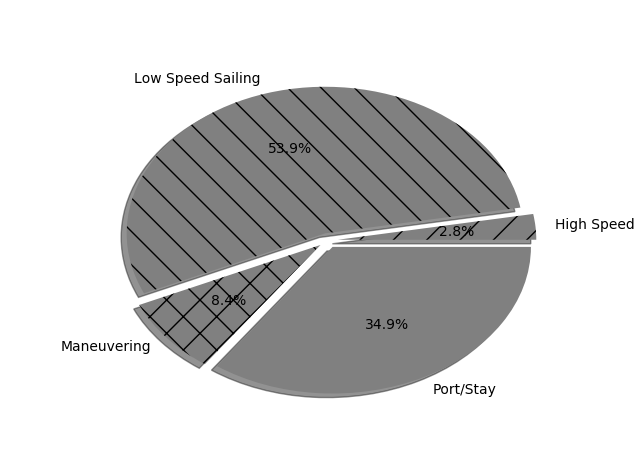
\includegraphics[width=0.8\linewidth]{Figures/Pie_operationalMode}
	\caption{Operational time by mode}
	\label{fig:opMode_pie}
\end{figure}

\begin{figure}[htbp]
	\centering
	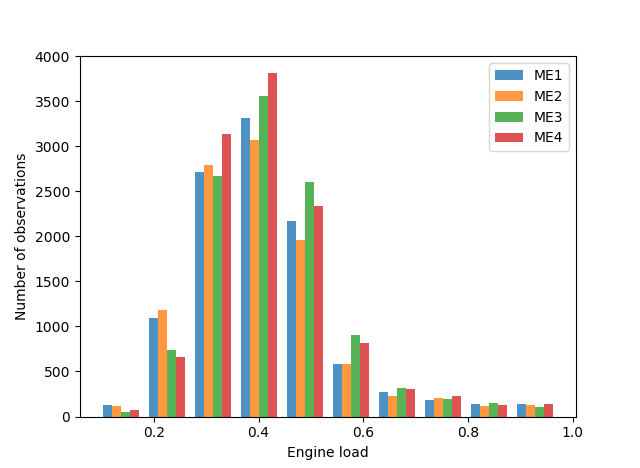
\includegraphics[width=0.8\linewidth]{Figures/Hist_mainEngines}
	\caption{Yearly load distribution, main engines}
	\label{fig:loadME_hist}
\end{figure}

\begin{figure}[htbp]
	\centering
	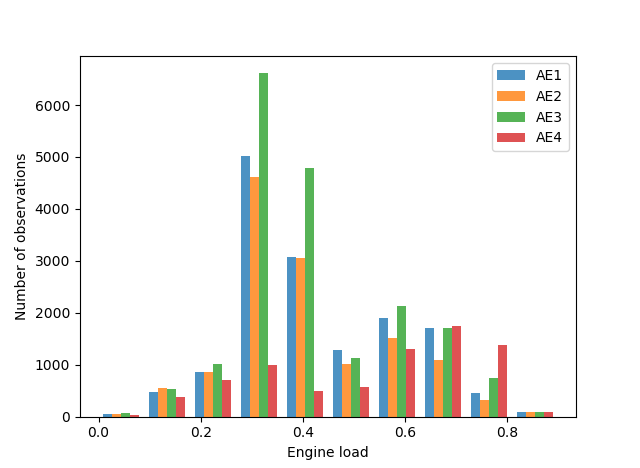
\includegraphics[width=0.8\linewidth]{Figures/Hist_auxEngines}
	\caption{Yearly load distribution, auxiliary engines}
	\label{fig:loadAE_hist}
\end{figure}

ANYTHING ELSE THAT CAN BE INTERESTING TO SHOW IN THE EXPLORATORY DATA ANALYSIS?




\subsection{Energy analysis} \label{sec:res:energy}

The ship energy demand is first subdivided among three main consumer categories: propulsion, electric power, and heat. The evolution of these demands over time during a typical voyage is shown in Figures \ref{fig:Demand_vs_time_W} and \ref{fig:Demand_vs_time_S}, representing a winter and a summer day respectively. It can be seen clearly how, as expected, the heating demand in winter is higher than in summer [2800-4500 kW vs 1100-2900 kW], as a consequence of the reduced need for compartment heating. On the other hand, the electric power demand behaves inversely, ranging around 1900 kW during the reference winter day (peaks are connected to the use of thrusters in port for maneuvering) and around 2300 kW during the reference summer day, where the difference is mostly associated to the demand of the HVAC compressors. Looking at the yearly cumulated demand, nearly 50\% of the total energy demand is related to ship propulsion (see Figure \ref{fig:Pie_EnergyDemand}), while the remaining portion is approximately equally split between electric energy and heat demand.



\begin{figure}[htbp]
	\centering
	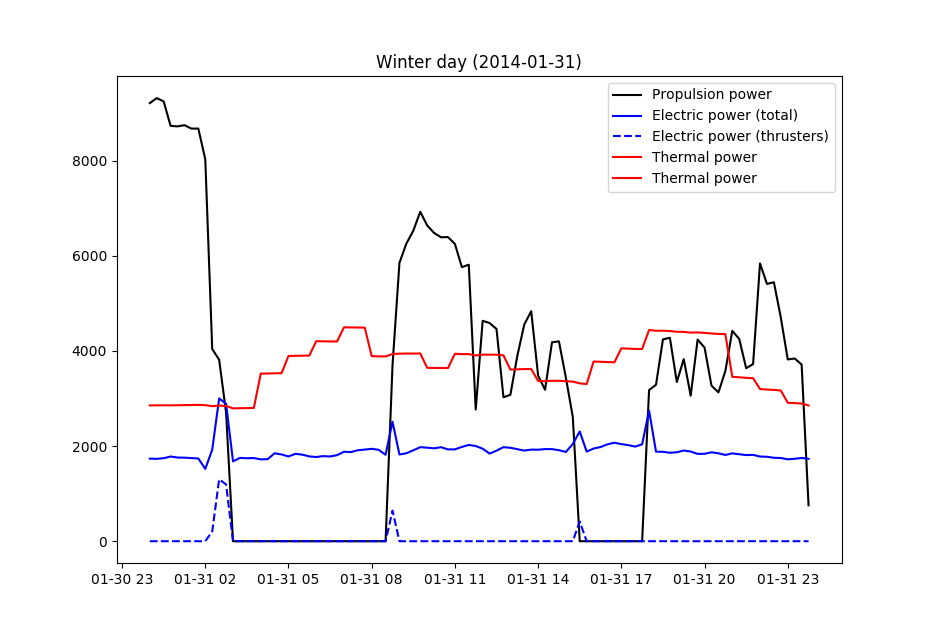
\includegraphics[width=0.9\linewidth]{Figures/Demand_vs_time_W}
	\caption{Energy demand during a day of operations, Winter (31 Jan)}
	\label{fig:Demand_vs_time_W}
\end{figure}

\begin{figure}[htbp]
	\centering
	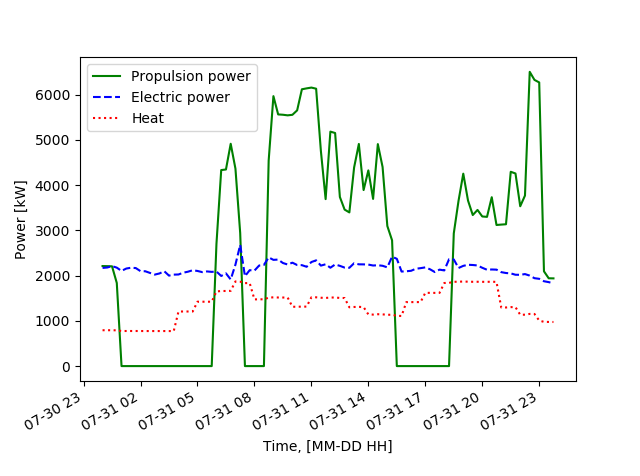
\includegraphics[width=0.9\linewidth]{Figures/Demand_vs_time_S}
	\caption{Energy demand during a day of operations, Summer (31 Jul)}
	\label{fig:Demand_vs_time_S}
\end{figure}

\begin{figure}[htbp]
	\centering
	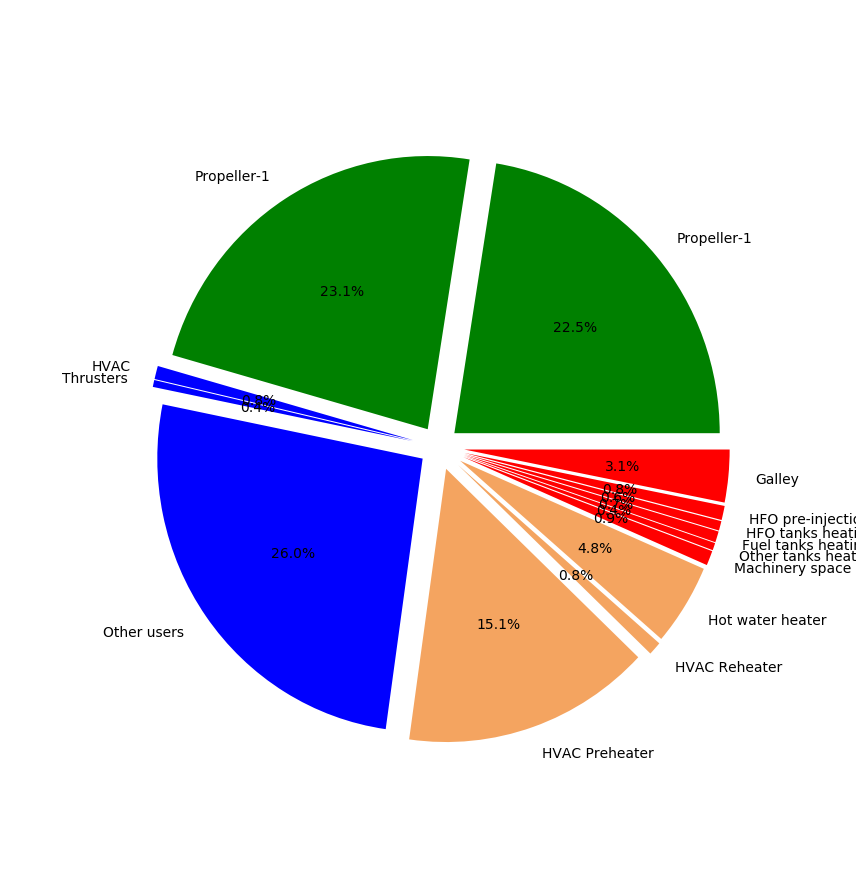
\includegraphics[width=0.9\linewidth]{Figures/Pie_EnergyDemand}
	\caption{Energy demand, aggregated data for one year of operations}
	\label{fig:Pie_EnergyDemand}
\end{figure}

\begin{figure}
	\centering
	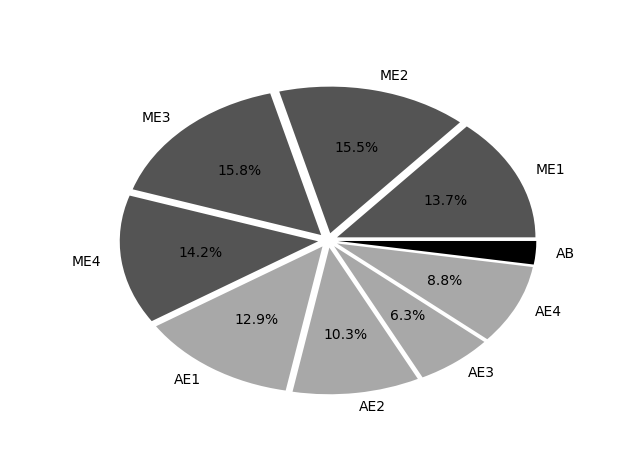
\includegraphics[width=0.9\linewidth]{Figures/Pie_EnergyGeneration}
	\caption{Energy generation, aggregated data for one year of operations}
	\label{fig:Pie_EnergyGeneration}
\end{figure}


Within the electric energy demand, the HVAC systems only represent a minor contribution (3\%), as it is only present for a few months during summer. This is not surprising, since it can be observed that (see Figure \ref{fig:TseaTairDIST}) the air is always below 27$^o$C, and rarely above 17$^o$C. Also the thrusters, although their instantaneous power demand is high, are only used for a very short time each day and, hence, their total contribution to the ship electrical energy demand is limited to 1.5\%. 

Heat recovery has a large impact on the overall heat demand (see Fig.  \ref{fig:Pie_HeatGeneration}). The the exhaust gas boilers and the heat recovery on the HT-water fulfill almost 75\% of the yearly demand for heating, leaving only the remaining 25\% to be provided by oil-fired auxiliary boilers. The contribution of the HRSG and the HTHR is substantially constant throughout the year (Fig. \ref{fig:TimeSeries_HeatGeneration}), while the auxiliary boilers are used to cover the peaks and the winter increased baseload. 

\begin{figure}
	\centering
	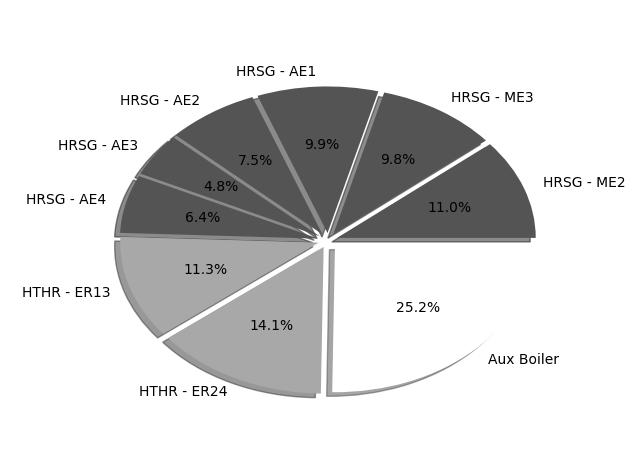
\includegraphics[width=0.99\linewidth]{Figures/Pie_HeatGeneration}
	\caption{Share of thermal power generated from on board heat systems}
	\label{fig:Pie_HeatGeneration}
\end{figure}

\begin{figure}
	\centering
	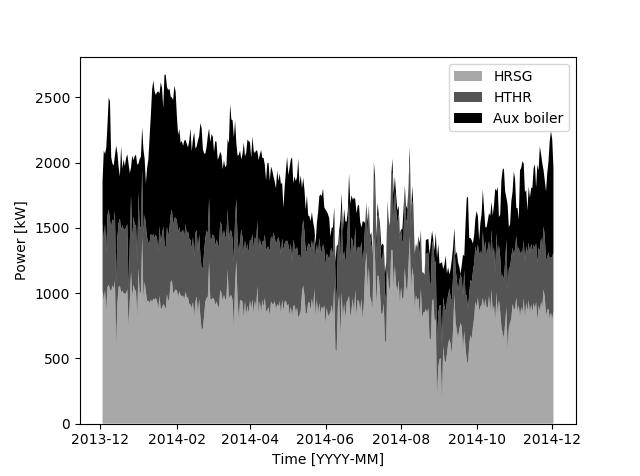
\includegraphics[width=0.99\linewidth]{Figures/TimeSeries_HeatGeneration}
	\caption{Time series representation of the thermal power generated from on board heat systems}
	\label{fig:TimeSeries_HeatGeneration}
\end{figure}


Looking at heating from the demand side, it can be seen that the HVAC pre-heater represents the largest contributor (56\%) to the annual heating demand, followed by the hot water heater (18\%) and by the galley (11\%).In multi-season central HVAC systems the pre-heater is generally used for the main heating contribution during winter, while the re-heater is only used for peak demand, or for adjusting the delivery air temperature during summer, thus explaining the large contribution of the former. The relatively large share of the hot water heater can instead be related to the fact that these systems are used during all seasons.

The full Sankey diagram representation of the energy flows on board is provided in Figure \ref{fig:Sankey}. 

\begin{figure}
	\centering
	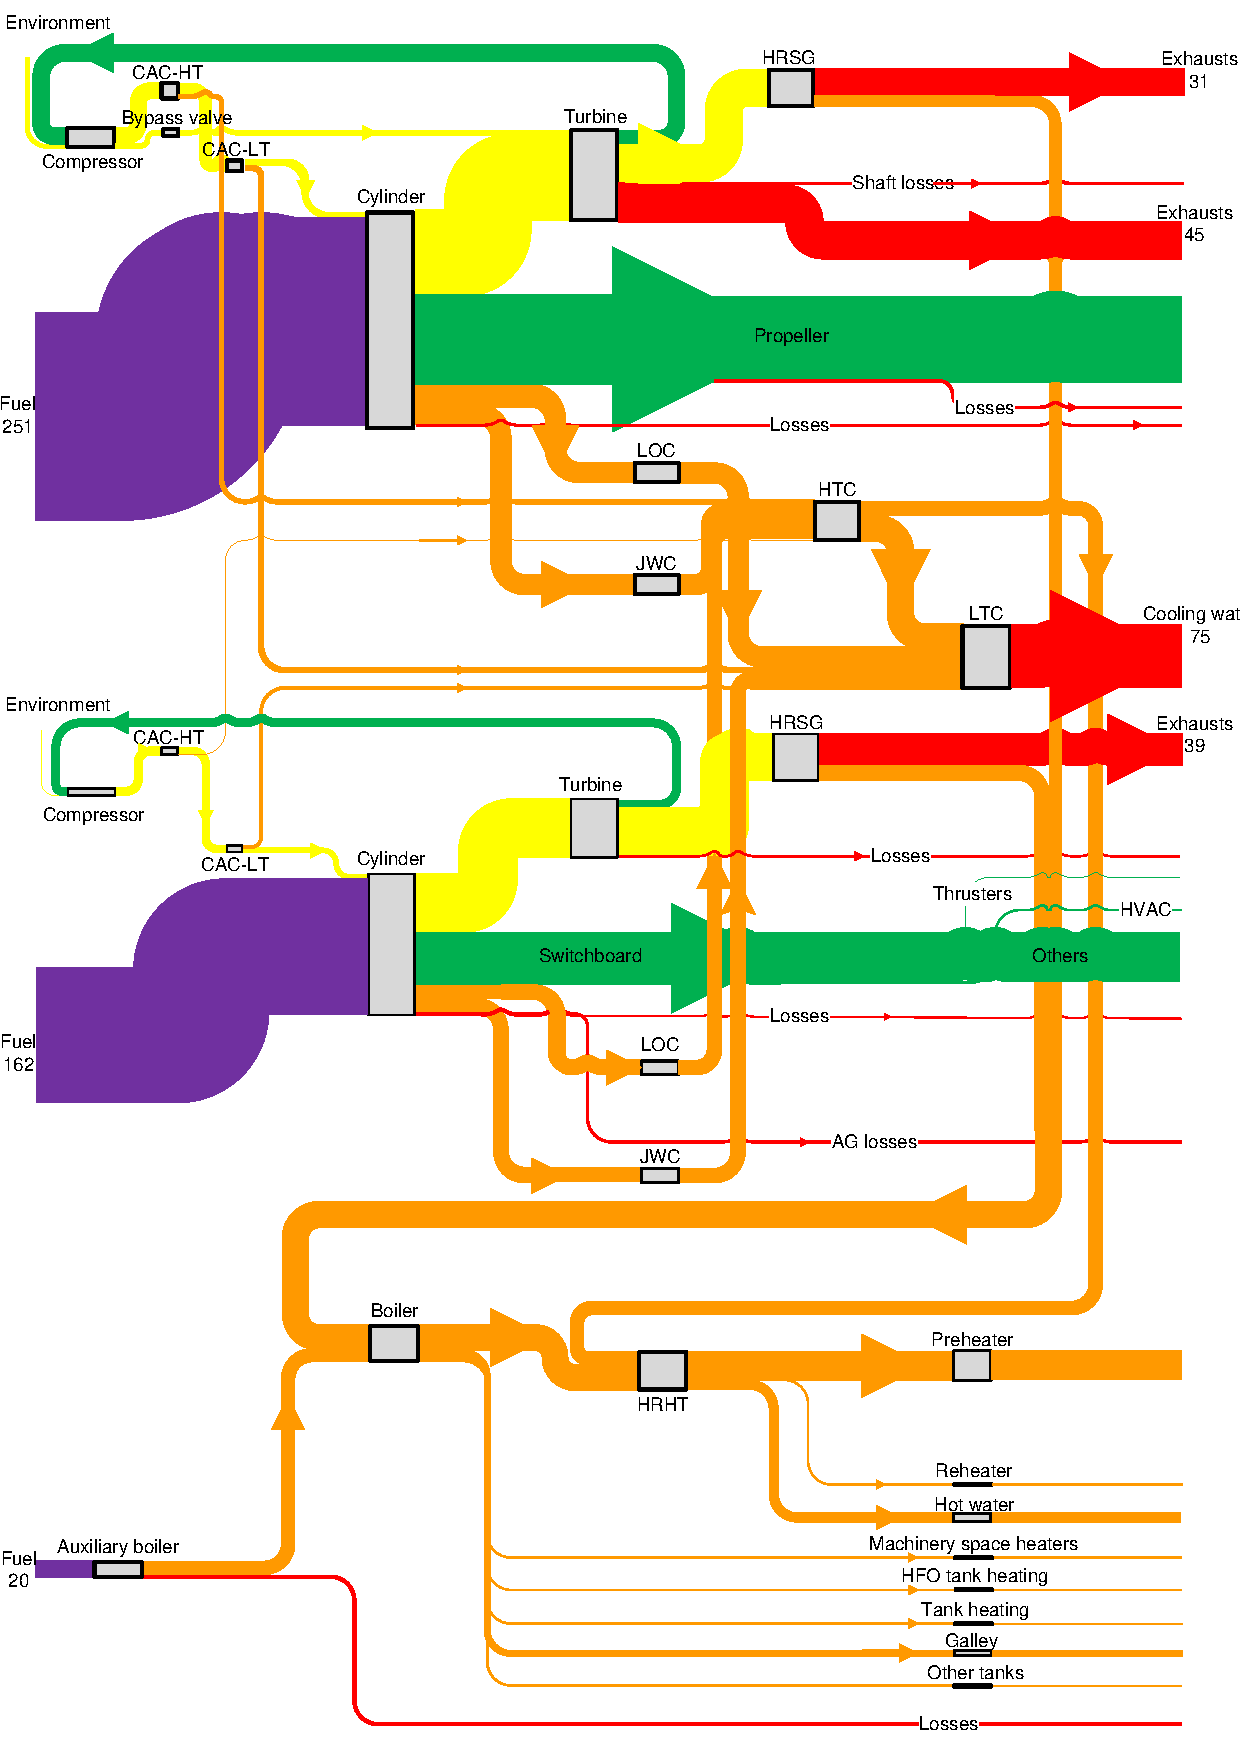
\includegraphics[width=0.99\linewidth]{Figures/Sankey_diagram_energy_ship_v9}
	\caption{Sankey diagram}
	\label{fig:Sankey}
\end{figure}





\subsection{Exergy Analysis} \label{sec:res:exergy}

The results of the exergy analysis of the ship energy systems are shown in Figure REF and Tables REF to REF. 
\begin{itemize}
	\item Table(s) --> Exergy efficiencies
	\begin{itemize}
		\item General at system level
		\item One per system (MEs, AEs, CoolingSystems, SteamSystems) 
	\end{itemize}
	\item Figure --> Grassman diagram
\end{itemize}

\begin{figure}
	\centering
	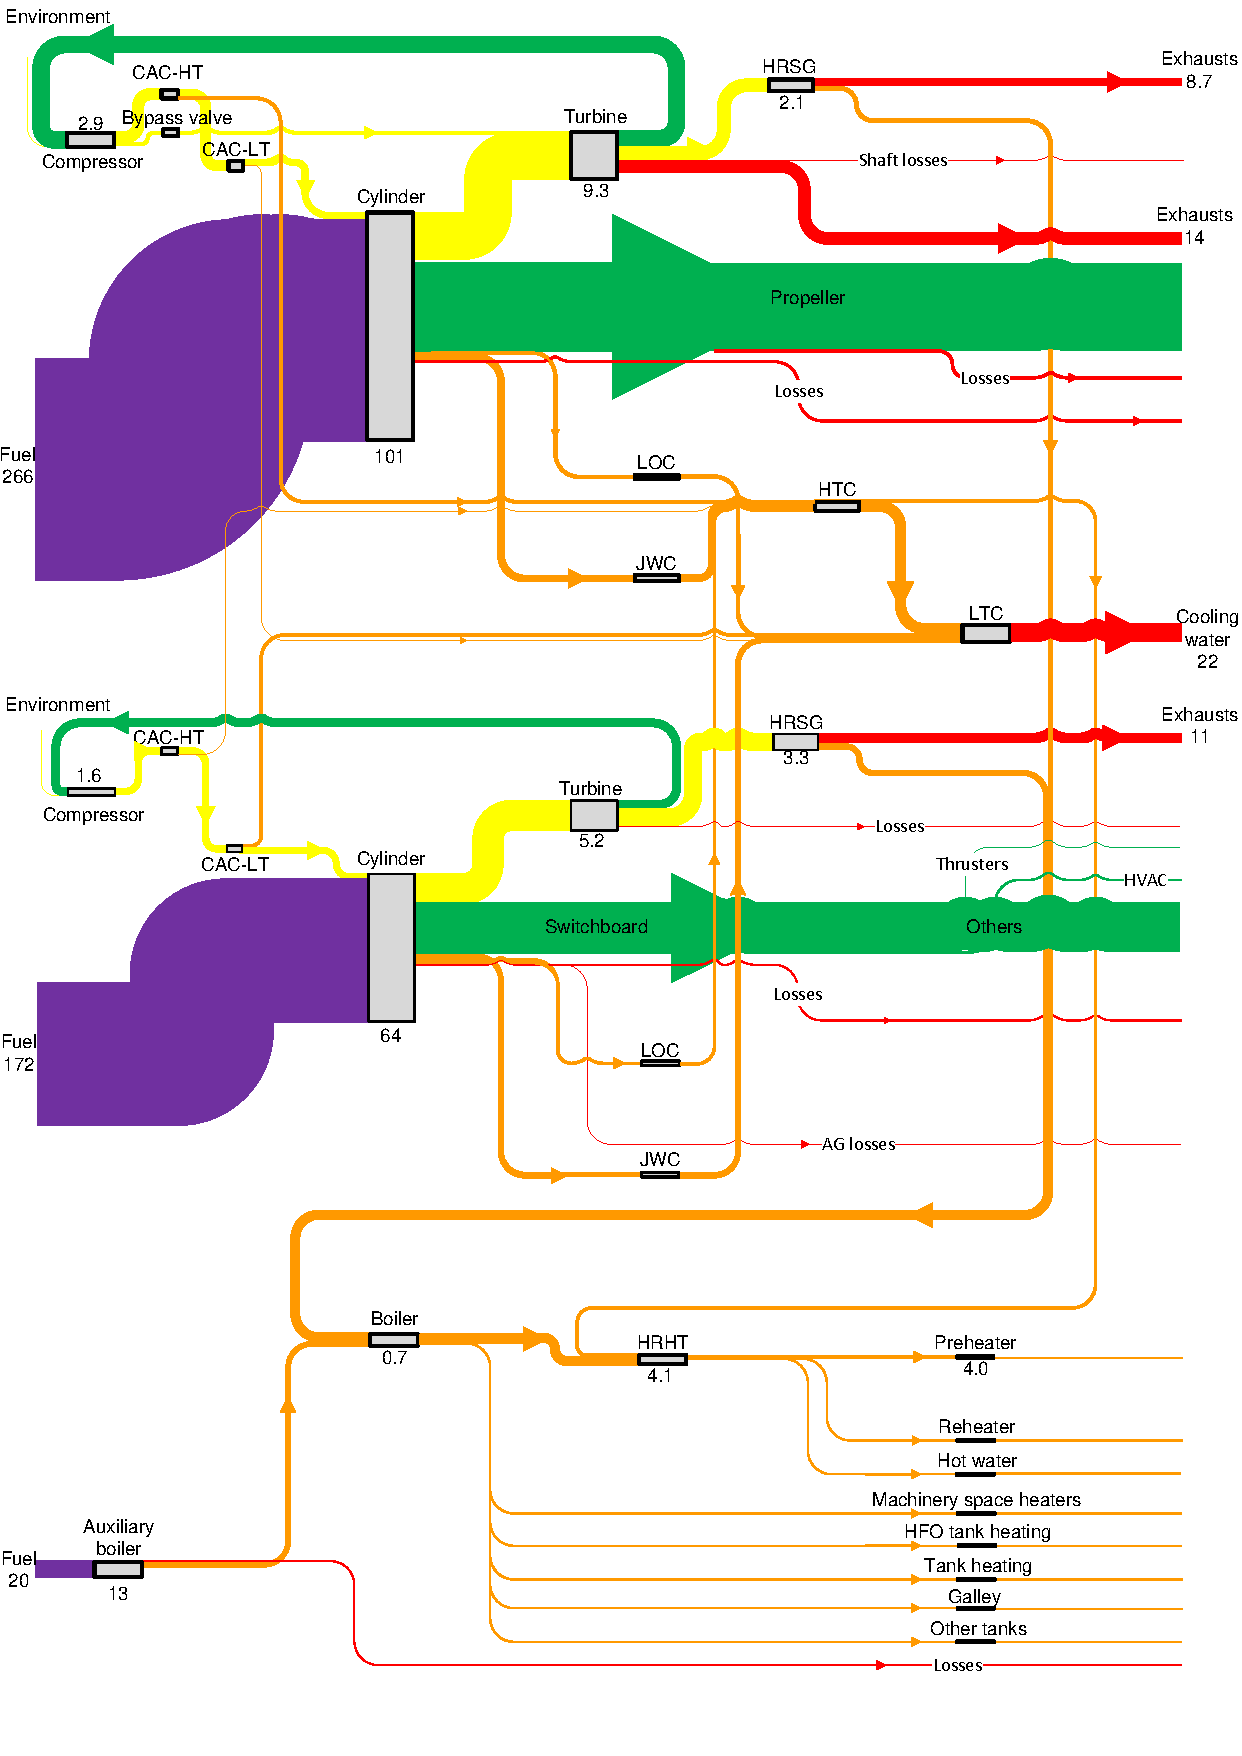
\includegraphics[width=0.99\linewidth]{Figures/Grassmann_diagram_v5}
	\caption{Grassmann diagram}
	\label{fig:Grassmann}
\end{figure}

It can be observed that there are large irreversibilities concentrated in some specific parts of the system that show potential for improvement. This is particularly the case of the LT/HT merging valves, where exergy is destroyed in the mixing process. Another substantial source of exergy destruction is the steam heater in the HTHR system, where heat at medium pressure (6 bar) is used to heat up water at 90$^o$C. The analysis of exergy destruction also points out the HVAC reheater as a potential source of improvement, based on the use of relatively high-temperature water for heating up air to around 30$^o$C and on the large energy demand of the component. Other important exergy destruction sources can be located in the engines, as expected, but the improvement of engine processes and technology goes beyond the scope of this work. 
\begin{table}
	\centering
	\begin{tabular}{cc}
		\hline 
		Component name & Contribution to exergy losses \\ 
		\hline 
		LT-HT merge & 13.4\% \\ 
		\hline 
		Sea water cooler & 10.6\% \\ 
		\hline 
		Steam heater & 6.0\% \\ 
		\hline 
		HVAC preheater & 6.0\% \\ 
		\hline 
	\end{tabular} 
	\caption{Major contributors to ship exergy losses. Losses related to combustion are not included in the calculation}
	\label{tab:exergyDestruction}
\end{table}

From the point of view of the exergy losses, it appears that the largest exergy losses are located in the exhaust gas. It should be noted that, even though a large part of this exergy cannot be recovered given the limitations on the exhaust gas outlet temperature to avoid the condensation of sulphuric acid, there is still a significant potential to be harvested if all the available exergy in the exhaust gas was recovered. This potential is further increased by the exergy destroyed in the process of dumping steam when it is produced in excess during summer. The exergy lost in the sea water coolers as low-temperature sea water discharged to the environment is lower, highlighting the fact that the potential for improving the efficiency of the system is located in other parts of the cooling systems. 

The efficiency of the recovery systems is also shown in Figure \ref{fig:Bar_efficiencyWHR}, where we show the fraction of the total energy (exergy) lost by the cooling systems and the exhaust gas of the ship's engines. It can be noted that, even when only looking at the energy that can be recovered based on the existing systems (i.e. not including the LT cooling systems, for instance), the recovery efficiency is located at around 25-35\% depending on whether the energy or the exergy efficiency is considered. Worth noting is also the fact that the efficiency on the exhaust gas side is lowered by the fact that two of the main engines are currently not equipped with HRSGs. 

\begin{figure}
	\centering
	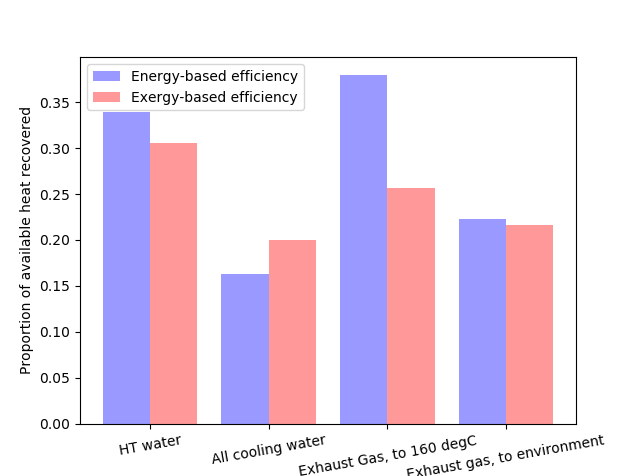
\includegraphics[width=0.99\linewidth]{Figures/Bar_WHRefficiency}
	\caption{Energy and exergy efficiency of the WHR systems}
	\label{fig:Bar_efficiencyWHR}
\end{figure}


\subsection{Typical operational days}  \label{sec:res:typicalDays}





\subsection{Potential for system improvement}

Based on the results of the energy and exergy analysis, it is possible to identify a number of possible measures that could potentially improve the efficiency of the system. 

Given the fact that many engines are operated at low load (both main and auxiliary engines), the system would benefit from both an electrification of the system and from the installation of batteries. The system electrification was explored by the authors \cite{Baldi2016b} and showed a relevant potential from both an environmental and an economic point of view. The installation of batteries was also considered in a previous publication by the authors \cite{Baldi2017} and proved the potential for yearly savings of 1-2\%. In this second case, however, it should be noted that the economic performance was not ensured. 

The availability of waste heat that is not already recovered by the system suggests that the system could benefit from the installation of a Heat-to-power WHR. This possibility was tested by the authors both in the case that no additional retrofit is performed \cite{Ahlgren2016,Mondejar2017}, with estimated savings of 22\% of the auxiliary power demand for a reference voyge, and in the case of a full integration with the rest of the system \cite{Baldi2017}, with estimated savings of up to 6\% of the total fuel consumption for a year of ship operations. 

It should be noted that in the second case the advantages in terms of system performance were obtained through a system-wide optimization of the system, where an improved utilization of the low-temperature waste heat available allowed "freeing" part of the high-temperature heat from the exhaust gas to the heat-to-power WHR system, hence improving the overall exergy efficiency of the system. This includes, for instance, the concept of using heat from the LT cooling systems (currently unused) for the HVAC preheater, hence reducing exergy destruction in the HVAC preheater itself and in the steam heater. This concept could be extended to other low-temperature heat consumers (such as the machinery space heating), but it would clearly constitute a larger benefit if applied to the HVAC preheater, which is the largest heat demand on board. 

Add reduction of non-HVAC el demand. Say absorption chillers are useless



\section{Conclusion}
\label{sec:conclusion}















\appendix

\section{Engine modelling, figures and tables}



\begin{figure}
	\centering
	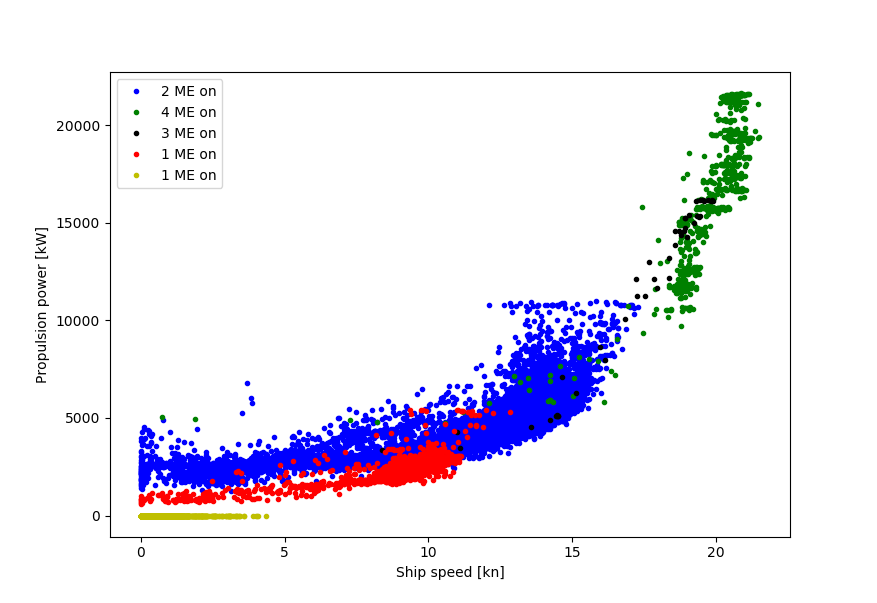
\includegraphics[width=0.9\linewidth]{Figures/Pme_vs_vship_Neng}
	\caption{Scatter plot, Propulsion power versus ship speed}
	\label{fig:Pme_vs_vship_Neng}
\end{figure}

\begin{figure}
	\centering
	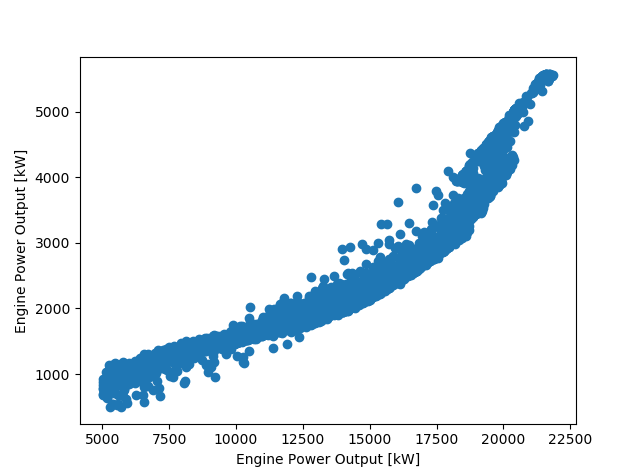
\includegraphics[width=0.9\linewidth]{Figures/Scatter_Pme_vs_TCspeed}
	\caption{Scatter plot, Main engine power versus turbocharger speed (ME1)}
	\label{fig:Pme_vs_TCspeed}
\end{figure}


\begin{table}
	\small
	\centering
	\begin{tabular}{llccrrrr}
		\hline
		\multicolumn{2}{l}{Variable} & Unit & M/C & 30\% & 50\% & 70\% & 90\% \\
		\hline
		\multicolumn{2}{l}{Compressor} & & & & & & \\ 
		& 	$T_{air,in}$  		& $^o$C & M & \multicolumn{4}{c}{302} \\ 
		&	$T_{air,out}$  		& $^o$C & C  & 356.0 & 409.4 & 434.1 & 461.7 \\ 
		&	$\dot{m}_{air}$  	& $kg/s$ & C  & 4.24 & 7.62 & 8.51 & 10.28 \\
		&   $\beta_{comp}$		& - 	& M & & & &  \\
		\multicolumn{2}{l}{Turbine} & & & & & &  \\
		&	$T_{eg,in}$   		& $^o$C & C  & 698.8 & 702.2 & 763.3 & 786.0 \\ 
		&	$T_{eg,out}$  		& $^o$C & M  & 639.3 & 592.9 & 633.2 & 631.0 \\ 
		&	$\dot{m}_{eg}$  	& $kg/s$ & C  & 4.35 & 7.79 & 8.73 & 10.57 \\
		&   $\beta_{exp}$		& - 	& C & & & &  \\
		\multicolumn{2}{l}{Bypass valve} & & & & & &  \\
		&	$\dot{m}_{air,BP}$	& $kg/s$ & C  & 0.98 & 2.05 & 1.02 & 0.39 \\  
		\multicolumn{2}{l}{Cylinders} & & & & & &   \\
		&	$\dot{m}_{air,in}$  & $kg/s$ & C  & 3.25 & 5.57 & 7.49 & 9.89 \\
		&	$\dot{m}_{fuel,in}$ & $kg/s$ & C  & 0.11 & 0.17 & 0.22 & 0.28 \\ 
		&	$\dot{m}_{eg,out}$  & $kg/s$ & C  & 3.37 & 5.74 & 7.71 & 10.17 \\
		&	$T_{air,in}$  		& $^o$C & M  & 323.7 & 323.2 & 323.1 & 323.5 \\ 
		&	$T_{eg,out}$  		& $^o$C & M  & 698.8 & 702.2 & 763.3 & 786.0 \\ 
		\multicolumn{2}{l}{CAC-LT stage} & & & & & &  \\
		&	$T_{air,in}$  		& $^o$C & C  & 355.2 & 350.1 & 360.0 & 368.7 \\ 
		&	$T_{air,out}$ 		& $^o$C & M  & 323.7 & 323.2 & 323.1 & 323.5 \\
		&	$T_{w,in}$   		& $^o$C & M  & 309.3 & 309.6 & 309.5 & 309.6 \\
		&	$T_{w,out}$   		& $^o$C & C  & 310.4 & 311.0 & 311.8 & 313.0 \\  
		& 	$\dot{m}_{w,LT}$  	& $kg/s$ & C& 23.36 & 26.09 & 29.1 & 31.53 \\
		\multicolumn{2}{l}{CAC-HT stage} & & & & & & \\
		&	$T_{air,in}$   		& $^o$C & C  & 356.0 & 409.4 & 434.1 & 461.7 \\
		&	$T_{air,out}$   	& $^o$C & C  & 355.2 & 350.1 & 360.0 & 368.7 \\ 
		&	$T_{w,in}$    		& $^o$C & C  & 360.8 & 360.2 & 359.6 & 358.7 \\ 
		&	$T_{w,out}$   		& $^o$C & C  & 360.8 & 362.6 & 363.6 & 365.4 \\
		& 	$\dot{m}_{w,HT}$  	& $kg/s$ & C & 33.21 & 33.18 & 33.33 & 33.33 \\
		\multicolumn{2}{l}{LOC} & & & & & &  \\
		&	$T_{lo,in}$   		& $^o$C & C  &346.6 & 348.9 & 349.8 & 350.5 \\ 
		&	$T_{lo,out}$    	& $^o$C & M  & 335.1 & 336.8 & 338.1 & 338.3 \\ 
		&	$T_{w,in}$    		& $^o$C & C  & 310.4 & 311.0 & 311.8 & 313.0 \\
		&	$T_{w,out}$   		& $^o$C & C  & 317.4 & 317.6 & 317.5 & 318.5 \\ 
		\multicolumn{2}{l}{JWC} & & & & & &  \\
		&	$T_{wall}$    		& $^o$C & C  & \multicolumn{4}{c}{423}  \\ 
		&	$T_{w,in}$    		& $^o$C & M  & 358.1 & 358.4 & 357.6 & 356.4 \\ 
		&	$T_{w,out}$	   		& $^o$C & C  & 360.8 & 360.2 & 359.6 & 358.7 \\ 
		\hline
	\end{tabular}
	\caption{Main engines, measured and calculated temperatures and flows at different engine loads}
	\label{tab:ME_values}
\end{table}


\begin{table}
	\small
	\centering
	\begin{tabular}{llccrrrr}
		\hline
		\multicolumn{2}{l}{Variable} & Unit & M/C & 30\% & 50\% & 70\% & 90\% \\
		\hline
		\multicolumn{2}{l}{Compressor} & & & & & & \\ 
		& 	$T_{air,in}$  		& $^o$C & M & 284.2 & 285.3 & 284.9 & 294.6 \\ 
		&	$T_{air,out}$  		& $^o$C & C  & 323.2 & 357.9 & 391.6 & 430.9 \\
		&	$\dot{m}_{air}$  	& $kg/s$ & C  & 1.96 & 2.65 & 3.5 & 4.27 \\
		&   $\beta_{comp}$		& - 	& M & & & &  \\
		\multicolumn{2}{l}{Turbine} & & & & & &  \\
		&	$T_{eg,in}$   		& $^o$C & M  & 729.5 & 762.1 & 770.3 & 798.5 \\
		&	$T_{eg,out}$  		& $^o$C & M  & 652.8 & 667.8 & 654.2 & 659.4 \\
		&	$\dot{m}_{eg}$  	& $kg/s$ & C  & 2.02 & 2.74 & 3.61 & 4.41 \\
		&   $\beta_{exp}$		& - 	& C & & & &  \\
		\multicolumn{2}{l}{Cylinders} & & & & & &   \\
		&	$\dot{m}_{air,in}$  & $kg/s$ & C  & 1.96 & 2.65 & 3.5 & 4.27 \\ 
		&	$\dot{m}_{fuel,in}$ & $kg/s$ & C  & 0.05 & 0.08 & 0.11 & 0.14 \\
		&	$\dot{m}_{eg,out}$  & $kg/s$ & C  & 2.02 & 2.74 & 3.61 & 4.41 \\
		&	$T_{air,in}$  		& $^o$C & M  & 320.8 & 322.3 & 327.6 & 329.1 \\
		&	$T_{eg,out}$  		& $^o$C & C  & 729.5 & 762.1 & 770.3 & 798.5 \\
		\multicolumn{2}{l}{CAC-LT stage} & & & & & &  \\
		&	$T_{air,in}$  		& $^o$C & C  & 323.2 & 356.3 & 366.7 & 372.0 \\ 
		&	$T_{air,out}$ 		& $^o$C & M  & 320.8 & 322.3 & 327.6 & 329.1 \\ 
		&	$T_{w,in}$   		& $^o$C & M  & 317.1 & 316.3 & 317.5 & 314.1 \\
		&	$T_{w,out}$   		& $^o$C & C  & 317.2 & 318.2 & 320.5 & 318.3 \\
		& 	$\dot{m}_{w,LT}$  	& $kg/s$ & C & 11.16 & 11.16 & 10.98 & 10.78 \\ 
		\multicolumn{2}{l}{CAC-HT stage} & & & & & & \\
		&	$T_{air,in}$   		& $^o$C & C  & 323.2 & 357.9 & 391.6 & 430.9 \\ 
		&	$T_{air,out}$   	& $^o$C & C  & 323.2 & 356.3 & 366.7 & 372.0 \\ 
		&	$T_{w,in}$    		& $^o$C & C  & 362.5 & 364.2 & 368.0 & 368.2 \\
		&	$T_{w,out}$   		& $^o$C & C  & 362.5 & 364.3 & 369.3 & 371.9 \\
		& 	$\dot{m}_{w,HT}$  	& $kg/s$ & C & 16.66 & 16.67 & 16.55 & 16.67 \\
		\multicolumn{2}{l}{LOC} & & & & & &  \\
		&	$T_{lo,in}$   		& $^o$C & C  & 348.2 & 350.3 & 354.0 & 357.3 \\
		&	$T_{lo,out}$    	& $^o$C & M  & 336.6 & 337.4 & 339.7 & 340.4 \\
		&	$T_{w,in}$    		& $^o$C & C & 317.2 & 318.2 & 320.5 & 318.3 \\ 
		&	$T_{w,out}$   		& $^o$C & C  & 325.9 & 327.8 & 331.4 & 331.3 \\
		\multicolumn{2}{l}{JWC} & & & & & & \\
		&	$T_{wall}$    		& $^o$C & C  & \multicolumn{4}{c}{423}  \\
		&	$T_{w,in}$    		& $^o$C & M  & 360.0 & 359.7 & 362.3 & 361.5 \\
		&	$T_{w,out}$	   		& $^o$C & C  & 362.5 & 364.2 & 368.0 & 368.2 \\  
		\hline
	\end{tabular}
	\caption{Auxiliary engines, measured and calculated temperatures and flows at different engine loads}
	\label{tab:AE_values}
\end{table}

\begin{table}
	\small
	\centering
	\begin{tabular}{lcrrrr}
		\hline
		Energy flow & type & 30\% & 50\% & 70\% & 90\% \\
		\hline
		Power output & Mech &  1767 & 2946 & 4118 & 5293 \\	
		Exhaust gas (after turbine) & Heat & 1672 & 2566 & 3227 & 3938 \\
		CAC-LT & Heat & 80 & 197 & 353 & 613 \\
		CAC-HT & Heat & 0 & 256  & 470 & 763  \\
		JWC & Heat & 501 & 507 & 549 & 620 \\
		LOC & Heat & 501 & 507 & 549 & 620 \\
		\hline
	\end{tabular}
	\caption{Main engines, energy flows at different engine loads}
	\label{tab:ME_flows}
\end{table}

\begin{table}
	\small
	\centering
	\begin{tabular}{lcrrrr}
		\hline
		Energy flow & type & 30\% & 50\% & 70\% & 90\% \\
		\hline
		Power output & Mech & 828 & 1381 & 1932 & 2482 \\
		
		Exhaust gas (after turbine) & Heat & 808 & 1144 & 1456 & 1753 \\
		CAC-LT & Heat & 5 & 92 & 139 & 185 \\
		CAC-HT & Heat & 0 & 4 & 87 & 256  \\
		JWC & Heat & 278 & 366 & 436 & 510 \\ 
		LOC & Heat & 278 & 366 & 436 & 510 \\ 
		\hline
	\end{tabular}
	\caption{Auxiliary engines, energy flows at different engine loads}
	\label{tab:AE_flows}
\end{table}

\section{Full tables of energy and exergy flows}

\subsection{Exergy flows}

\begin{table}
	\centering
	\begin{tabular}{clclcrrrrrrrr}
\toprule
\multicolumn{2}{c}{From} & \multicolumn{2}{c}{To}  & Type & Total & Port/Stay & Low Speed Sailing & Maneuvering & High Speed Sailing & Winter & Mid-Season & Summer\\
\midrule
E & Env. & ME & Comp. & Ph & 0.16 & 0.000 & 0.141 & 0.013 & 0.010 & 0.102 & 0.048 & 0.014\\
ME & Comp. & ME & CAC-HT & Ph & 13.64 & 0.004 & 9.932 & 1.148 & 2.555 & 4.976 & 5.626 & 3.037\\
ME & CAC-HT & ME & CAC-LT & Ph & 12.20 & 0.004 & 9.008 & 1.023 & 2.164 & 4.476 & 5.079 & 2.643\\
ME & CAC-LT & ME & Cyl. & Ph & 11.04 & 0.004 & 8.144 & 0.932 & 1.960 & 4.019 & 4.619 & 2.401\\
ME & Turb. & ME & Comp. & W & 20.16 & 0.006 & 15.287 & 1.659 & 3.207 & 7.539 & 8.523 & 4.098\\
ME & Cyl. & ME & Turb. & Ph & 55.91 & 0.037 & 43.951 & 4.839 & 7.085 & 22.177 & 23.408 & 10.327\\
ME & Turb. & E & HRSG & Ph & 15.45 & 0.014 & 12.621 & 1.353 & 1.458 & 6.605 & 6.320 & 2.520\\
ME & Turb. & E & Losses & Q & 0.81 & 0.001 & 0.653 & 0.069 & 0.087 & 0.341 & 0.338 & 0.131\\
ME & Turb. & E & Env. & Ph & 14.04 & 0.014 & 11.256 & 1.285 & 1.489 & 5.694 & 5.941 & 2.409\\
ME & Comp. & ME & BP valve & Ph & 17.44 & 0.004 & 13.179 & 1.425 & 2.831 & 6.557 & 7.323 & 3.559\\
ME & BP valve & ME & Turb. & Ph & 3.80 & 0.001 & 3.246 & 0.277 & 0.275 & 1.581 & 1.697 & 0.522\\
ME & CAC-HT & CS & HT Cool. & Q & 1.16 & 0.000 & 0.924 & 0.125 & 0.392 & 0.501 & 0.547 & 0.394\\
ME & CAC-LT & CS & LT Cool. & Q & 0.59 & 0.000 & 0.864 & 0.091 & 0.203 & 0.456 & 0.460 & 0.242\\
ME & Cyl. & ME & LOC & Q & 4.18 & 0.011 & 3.442 & 0.443 & 0.286 & 1.860 & 1.758 & 0.565\\
ME & Cyl. & ME & JWC & Q & 8.13 & 0.022 & 6.660 & 0.879 & 0.565 & 3.424 & 3.514 & 1.188\\
ME & JWC & CS & HT Cool. & Q & 5.30 & 0.022 & 6.660 & 0.879 & 0.565 & 3.424 & 3.514 & 1.188\\
ME & LOC & CS & LT Cool. & Q & 2.45 & 0.011 & 3.442 & 0.443 & 0.286 & 1.860 & 1.758 & 0.565\\
ME & Cyl. & E & Losses & Q & 0.63 & 0.002 & 0.525 & 0.067 & 0.040 & 0.275 & 0.271 & 0.088\\
ME & HRSG & S & Boiler & Q & 4.63 & 0.008 & 5.622 & 0.628 & 0.498 & 3.015 & 2.677 & 1.064\\
ME & HRSG & E & Env. & Ph & 8.69 & 0.006 & 6.999 & 0.725 & 0.961 & 3.590 & 3.643 & 1.456\\
ME & Cyl. & P & Prop. shaft & W & 107.39 & 0.141 & 85.158 & 10.141 & 11.947 & 42.238 & 45.916 & 19.233\\
ME & Fuel tank & ME & Cyl. & Ch & 266.02 & 0.382 & 212.237 & 25.450 & 27.949 & 105.146 & 114.197 & 46.675\\
ME & Fuel tank & ME & Cyl. & Q & 0.15 & 0.000 & 0.125 & 0.014 & 0.014 & 0.068 & 0.063 & 0.022\\
\midrule
E & Env. & AE & Comp. & Ph & 0.01 & 0.002 & 0.003 & 0.001 & 0.000 & 0.003 & 0.001 & 0.001\\
AE & Comp. & AE & CAC-HT & Ph & 7.91 & 2.960 & 4.008 & 0.659 & 0.288 & 3.392 & 3.091 & 1.432\\
AE & CAC-HT & AE & CAC-LT & Ph & 7.65 & 2.835 & 3.906 & 0.644 & 0.269 & 3.302 & 3.017 & 1.335\\
AE & CAC-LT & AE & Cyl. & Ph & 7.09 & 2.589 & 3.650 & 0.606 & 0.248 & 3.066 & 2.802 & 1.227\\
AE & Turb. & AE & Comp. & W & 9.54 & 3.504 & 4.853 & 0.841 & 0.338 & 4.087 & 3.762 & 1.687\\
AE & Cyl. & AE & Turb. & Ph & 36.26 & 11.776 & 19.815 & 3.592 & 1.079 & 15.705 & 14.961 & 5.597\\
AE & Turb. & E & HRSG & Ph & 21.04 & 6.378 & 11.936 & 2.157 & 0.571 & 9.166 & 8.866 & 3.011\\
AE & Turb. & E & Losses & Q & 0.46 & 0.132 & 0.259 & 0.060 & 0.012 & 0.209 & 0.194 & 0.060\\
AE & Comp. & AE & BP valve & Ph & 7.91 & 2.960 & 4.008 & 0.659 & 0.288 & 3.392 & 3.091 & 1.432\\
AE & BP valve & AE & Turb. & Ph & 0.00 & 0.000 & 0.000 & 0.000 & 0.000 & 0.000 & 0.000 & 0.000\\
AE & CAC-HT & CS & HT Cool. & Q & 0.24 & 0.125 & 0.102 & 0.015 & 0.018 & 0.090 & 0.074 & 0.097\\
AE & CAC-LT & CS & LT Cool. & Q & 0.36 & 0.245 & 0.256 & 0.037 & 0.021 & 0.236 & 0.215 & 0.108\\
AE & Cyl. & AE & LOC & Q & 3.14 & 0.962 & 1.757 & 0.344 & 0.075 & 1.476 & 1.275 & 0.388\\
AE & Cyl. & AE & JWC & Q & 5.84 & 1.772 & 3.270 & 0.656 & 0.144 & 2.608 & 2.451 & 0.783\\
AE & JWC & CS & HT Cool. & Q & 3.90 & 1.772 & 3.270 & 0.656 & 0.144 & 2.608 & 2.451 & 0.783\\
AE & LOC & CS & LT Cool. & Q & 2.18 & 0.962 & 1.757 & 0.344 & 0.075 & 1.476 & 1.275 & 0.388\\
AE & Cyl. & E & Losses & Q & 0.37 & 0.096 & 0.217 & 0.047 & 0.008 & 0.166 & 0.159 & 0.044\\
AE & HRSG & S & Boiler & Q & 6.32 & 2.869 & 5.504 & 1.011 & 0.237 & 4.309 & 3.901 & 1.412\\
AE & HRSG & E & Env. & Ph & 11.42 & 3.509 & 6.432 & 1.145 & 0.334 & 4.857 & 4.965 & 1.599\\
AE & Cyl. & EL & SB & W & 62.02 & 20.781 & 34.328 & 6.249 & 1.851 & 26.971 & 26.344 & 9.894\\
AE & Cyl. & E & AG losses & Q & 0.85 & 0.228 & 0.499 & 0.105 & 0.020 & 0.384 & 0.363 & 0.104\\
AE & Fuel tank & AE & Cyl. & Ch & 172.09 & 54.452 & 94.876 & 17.916 & 4.849 & 73.199 & 72.744 & 26.150\\
AE & Fuel tank & AE & Cyl. & Q & 0.08 & 0.019 & 0.054 & 0.009 & 0.003 & 0.041 & 0.033 & 0.010\\
\midrule
CS & HT Cool. & CS & LT Cool. & Q & 7.36 & 1.46 & 8.63 & 1.36 & 0.97 & 5.10 & 5.25 & 2.08\\
CS & HT Cool. & S & HRHT & Q & 3.24 & 0.46 & 2.33 & 0.31 & 0.14 & 1.53 & 1.34 & 0.38\\
S & Boiler & S & HRHT & Q & 10.87 & 4.94 & 5.09 & 0.75 & 0.09 & 6.51 & 3.82 & 0.53\\
S & Aux Boiler & S & Boiler & Ph & 5.71 & 4.66 & 0.90 & 0.17 & -0.03 & 3.77 & 1.85 & 0.10\\
S & Aux Boiler & E & Env. & Ph & 1.51 & 1.04 & 0.38 & 0.08 & 0.00 & 0.99 & 0.50 & 0.03\\
S & Fuel tank & S & Aux Boiler & Ch & 20.12 & 14.37 & 4.73 & 1.02 & 0.01 & 12.99 & 6.76 & 0.37\\
S & HRHT & D & HVAC-PH & Q & 7.43 & 1.22 & 1.89 & 0.25 & 0.05 & 2.29 & 1.11 & 0.00\\
S & HRHT & D & HVAC-RH & Q & 0.33 & 0.09 & 0.13 & 0.03 & 0.03 & 0.00 & 0.00 & 0.28\\
S & HRHT & D & HWH  & Q & 2.27 & 0.64 & 1.09 & 0.17 & 0.05 & 0.84 & 0.81 & 0.31\\
S & Boiler & D & MSH & Q & 0.68 & 0.06 & 0.10 & 0.01 & 0.00 & 0.09 & 0.07 & 0.02\\
S & Boiler & D & HFO TH & Q & 0.66 & 0.13 & 0.20 & 0.03 & 0.01 & 0.16 & 0.16 & 0.04\\
S & Boiler & D & HFO H & Q & 0.44 & 0.04 & 0.21 & 0.03 & 0.02 & 0.13 & 0.12 & 0.04\\
S & Boiler & D & TH & Q & 0.51 & 0.08 & 0.12 & 0.02 & 0.01 & 0.11 & 0.10 & 0.03\\
S & Boiler & D & G & Q & 2.45 & 0.44 & 0.98 & 0.14 & 0.04 & 0.71 & 0.69 & 0.19\\
S & Boiler & D & OT & Q & 0.34 & 0.08 & 0.12 & 0.02 & 0.01 & 0.11 & 0.10 & 0.03\\
EL & SB & EL & Thrusters & W & 0.94 & 0.00 & 0.00 & 0.94 & 0.00 & 0.36 & 0.43 & 0.15\\
EL & SB & EL & HVAC & W & 1.79 & 0.59 & 0.85 & 0.18 & 0.18 & 0.00 & 0.00 & 1.79\\
EL & SB & EL & Other el. Dem. & W & 59.29 & 19.99 & 32.66 & 4.99 & 1.64 & 26.06 & 25.45 & 7.78\\
P & Prop. shaft & P & Prop. & W & 104.19 & 0.14 & 82.62 & 9.84 & 11.59 & 40.98 & 44.55 & 18.66\\
P & Prop. shaft & E & Losses & Q & 3.20 & 0.00 & 2.54 & 0.30 & 0.36 & 1.26 & 1.37 & 0.57\\
S & Boiler & E & Dumped steam & Q & 0.81 & 0.00 & 0.43 & 0.13 & 0.25 & 0.05 & 0.20 & 0.55\\
\midrule
& HVAC-PH & D & Dem. & Q & 3.41 & 1.22 & 1.89 & 0.25 & 0.05 & 2.29 & 1.11 & 0.00\\
& HVAC-RH & D & Dem. & Q & 0.28 & 0.09 & 0.13 & 0.03 & 0.03 & 0.00 & 0.00 & 0.28\\
& HWH  & D & Dem. & Q & 1.96 & 0.64 & 1.09 & 0.17 & 0.05 & 0.84 & 0.81 & 0.31\\
& MSH & D & Dem. & Q & 0.18 & 0.06 & 0.10 & 0.01 & 0.00 & 0.09 & 0.07 & 0.02\\
& HFO TH & D & Dem. & Q & 0.37 & 0.13 & 0.20 & 0.03 & 0.01 & 0.16 & 0.16 & 0.04\\
& HFO H & D & Dem. & Q & 0.29 & 0.04 & 0.21 & 0.03 & 0.02 & 0.13 & 0.12 & 0.04\\
& TH & D & Dem. & Q & 0.23 & 0.08 & 0.12 & 0.02 & 0.01 & 0.11 & 0.10 & 0.03\\
& G & D & Dem. & Q & 1.59 & 0.44 & 0.98 & 0.14 & 0.04 & 0.71 & 0.69 & 0.19\\
& OT & D & Dem. & Q & 0.15 & 0.05 & 0.08 & 0.01 & 0.00 & 0.07 & 0.07 & 0.02\\
\bottomrule
	\end{tabular}
\end{table}

\section{Full equation list}

\begin{table}[htbp]
	\centering
	\begin{tabular}{p{4cm}l}
		\hline
		\multirow{2}{*}{Before compressor}		& $ T_{comp,in} = $ Measured \\
												& $ p_{comp,in} = $ Measured \\
		\multirow{3}{*}{After compressor}		& $ T_{comp,out} = T_{comp,in} + \frac{T_{comp,out,is} - T_{comp,in} }{\eta_{comp,is}}  $  \\
												& $ p_{comp,out} = $ Measured \\
												& $ \eta_{comp,is} = P_2(\frac{p_{comp,out}}{p_{comp,in}}) $ \\
		\multirow{3}{*}{After CAC-HT stage}		& $ p_{CAC-HT,out} = p_{comp,out} $ \\
												& $ T_{CAC-HT,out} = T_{comp,out} - \frac{\dot{Q}_{CAC,HT}}{\dot{m}_{air,cyl}} $ \\
												& $ \dot{Q}_{CAC,HT} = P_2(\lambda) $ \\
		\multirow{3}{*}{After CAC-LT stage}		& $ p_{CAC-LT,out} = p_{comp,out} $ \\
												& $ T_{CAC-LT,out} = T_{CAC-HT,out} - \frac{\dot{Q}_{CAC,LT}}{\dot{m}_{air,cyl}} $ \\
												& $ \dot{Q}_{CAC,LT} = P_2(\lambda) $ \\
		\multirow{3}{*}{After CAC-LT stage}											
												
												
	\end{tabular}
\end{table}



\section{Full list of available measurements}

\bibliographystyle{unsrt}
\bibliography{bibliography}

%% \begin{thebibliography}{widestlabel}
%% \bibitem{label}
%% Text of bibliographic item
%%\end{thebibliography}

\end{document}
\endinput
%%
%% End of file `elsarticle-template-num.tex'.